\documentclass[12pt,a4paper,oneside,openany,graphicx]{report}

\usepackage{listings}
\usepackage{xcolor}

\usepackage{amsfonts}
\usepackage{amssymb}
\usepackage{fullpage}
\usepackage{textcomp}
\usepackage{chngcntr}
\usepackage{listings}
\usepackage{color}	
\usepackage{indentfirst}
\usepackage{setspace}
\usepackage{rotating}
\usepackage[utf8]{inputenc}
\usepackage{array}
\usepackage{placeins}
\usepackage{url}
\usepackage{tabularx}
\usepackage{lipsum}
\usepackage{caption}
\usepackage{ltablex}
											
\lstloadlanguages{C,C++,csh,Java}

\definecolor{red}{rgb}{0.6,0,0} 
\definecolor{blue}{rgb}{0,0,0.6}
\definecolor{green}{rgb}{0,0.8,0}
\definecolor{cyan}{rgb}{0.0,0.6,0.6}
\definecolor{cloudwhite}{rgb}{0.9412, 0.9608, 0.8471}
\lstset{
	language=csh,
	basicstyle=\footnotesize\ttfamily,
	numbers=left,
	numberstyle=\tiny,
	numbersep=5pt,
	tabsize=2,
	extendedchars=true,
	breaklines=true,
	frame=b,
	stringstyle=\color{blue}\ttfamily,
	showspaces=false,
	showtabs=false,
	xleftmargin=17pt,
	framexleftmargin=17pt,
	framexrightmargin=5pt,
	framexbottommargin=4pt,
	commentstyle=\color{green},
	morecomment=[l]{//}, %use comment-line-style!
	morecomment=[s]{/*}{*/}, %for multiline comments
	showstringspaces=false,
	morekeywords={ abstract, event, new, struct,
		as, explicit, null, switch,
		base, extern, object, this,
		bool, false, operator, throw,
		break, finally, out, true,
		byte, fixed, override, try,
		case, float, params, typeof,
		catch, for, private, uint,
		char, foreach, protected, ulong,
		checked, goto, public, unchecked,
		class, if, readonly, unsafe,
		const, implicit, ref, ushort,
		continue, in, return, using,
		decimal, int, sbyte, virtual,
		default, interface, sealed, volatile,
		delegate, internal, short, void,
		do, is, sizeof, while,
		double, lock, stackalloc,
		else, long, static,
		enum, namespace, string},
	keywordstyle=\color{cyan},
	identifierstyle=\color{red},
	backgroundcolor=\color{cloudwhite},
}

\usepackage{caption}
\DeclareCaptionFont{white}{\color{white}}
\DeclareCaptionFormat{listing}{\colorbox{blue}{\parbox{\textwidth}{\hspace{15pt}#3}}}
\captionsetup[lstlisting]{format=listing,labelfont=white,textfont=white, singlelinecheck=false, margin=0pt, font={bf,footnotesize}}																			

\usepackage[explicit]{titlesec}


\usepackage[top=1.5cm, bottom=2.2cm, left=3cm, right=2cm, headsep=1.2cm, footskip=1cm, margin=1in, headheight=0.3cm, textheight=24.5cm, textwidth=16cm]{geometry}
\usepackage{mathptmx}% http://ctan.org/pkg/mathptmx
\usepackage{iftex}
\ifXeTeX % Tectonic/XeLaTeX: use TeX Gyre Termes (Times) so the text matches the pdfLaTeX build
  \usepackage{fontspec}
  \setmainfont{texgyretermes}[Extension=.otf, UprightFont=*-regular, BoldFont=*-bold, ItalicFont=*-italic, BoldItalicFont=*-bolditalic]
\fi

\usepackage{fancyhdr}
\usepackage{array}
\usepackage{longtable}
\usepackage{graphicx}
\usepackage[utf8]{inputenc}
\usepackage[english]{babel}
\usepackage{float}

\usepackage{listings}
\textwidth 6.5in
\textheight 9.5in

\renewcommand{\arraystretch}{1.5}

\usepackage{fancyhdr}
\pagestyle{fancy}
\pagenumbering{roman}


\usepackage{subfigure}
\usepackage[toc,page]{appendix}
% ---- additions for the Sentinel report ----
\usepackage{amsmath}
\usepackage{booktabs}
\usepackage{multirow}
\usepackage{makecell}
\usepackage{algorithm}
\usepackage{algpseudocode}
\usepackage{pgfplots}
\pgfplotsset{compat=1.17}
\usepackage{etoolbox}
\usepackage[shortlabels]{enumitem}
\setlist{itemsep=2pt, topsep=4pt}
\counterwithin{figure}{chapter}
\counterwithin{table}{chapter}
\counterwithin{algorithm}{chapter}
\graphicspath{{Images/}}
\AtBeginEnvironment{algorithmic}{\setstretch{1.08}}
\AtBeginEnvironment{tabular}{\setstretch{1.0}}
\AtBeginEnvironment{longtable}{\setstretch{1.0}}
\captionsetup[figure]{skip=4pt}
\setlength{\intextsep}{8pt plus 2pt minus 2pt}
\renewcommand{\topfraction}{0.88}
\renewcommand{\bottomfraction}{0.6}
\renewcommand{\textfraction}{0.08}
\renewcommand{\floatpagefraction}{0.82}
\setcounter{topnumber}{3}
\setcounter{totalnumber}{4}

\setlength{\headheight}{15pt}
\lstdefinestyle{py}{language=Python, literate={“}{{``}}1 {”}{{''}}1 {’}{{'}}1 {≤}{{$\le$}}1 {–}{{--}}1 {—}{{---}}1 {→}{{$\to$}}1 {…}{{...}}1, basicstyle=\footnotesize\ttfamily\setstretch{1.0}, keywordstyle=\color{blue}\bfseries,
  identifierstyle=\color{black}, stringstyle=\color{red}\ttfamily, commentstyle=\color{gray}\itshape,
  morekeywords={self,True,False,None}, backgroundcolor=\color{cloudwhite}}
\lstdefinestyle{js}{literate={“}{{``}}1 {”}{{''}}1 {’}{{'}}1 {≤}{{$\le$}}1 {–}{{--}}1 {—}{{---}}1 {→}{{$\to$}}1 {…}{{...}}1, basicstyle=\footnotesize\ttfamily\setstretch{1.0}, identifierstyle=\color{black}, keywordstyle=\color{blue}\bfseries,
  stringstyle=\color{red}\ttfamily, backgroundcolor=\color{cloudwhite}, morekeywords={const,let,await,async,function,return,try,catch}}
\lstdefinestyle{json}{literate={“}{{``}}1 {”}{{''}}1 {’}{{'}}1 {≤}{{$\le$}}1 {–}{{--}}1 {—}{{---}}1 {→}{{$\to$}}1 {…}{{...}}1, basicstyle=\scriptsize\ttfamily\setstretch{1.0}, identifierstyle=\color{black}, keywordstyle=\color{black},
  stringstyle=\color{black}, backgroundcolor=\color{cloudwhite}, numbers=none}
% thebibliography should not start its own unnumbered chapter (References is Chapter 7)
\patchcmd{\thebibliography}{\chapter*{\bibname}}{}{}{}
\usepackage[hidelinks]{hyperref}
\begin{document}

\pagenumbering{roman}

\thispagestyle{empty}
\begin{center}

\textbf {{ \LARGE Sentinel: Social Media Threat Detection \& Security System \\ }}
\vspace{1pc}
\vspace{0.5pc}


{ \Large Submitted in partial fulfillment of the requirements  \\ for the degree of \\
					\vspace{1pc}
                          \textbf{B.E. Computer Engineering\\}
\vspace{1pc}
By\\

	\begin{table}[h]
\centering
\Large{
\begin{tabular}{>{\bfseries}lc>{\bfseries}r}
 Rayan Pawar & \textbf{41} & \textbf{232121} \\
 Vyom Desai & \textbf{48} & \textbf{232028} \\
 Neil Dias & \textbf{49} & \textbf{232030} \\
 Jason D'Souza & \textbf{53} & \textbf{232037}
\end{tabular}}
\end{table}
				\vspace{0.5pc}
			 Guide\\

			\textbf{Ms. Jewel Correia} \\
		              {[Designation]}\\
\vspace{1pc}
\begin{figure}[H]
\centering

\includegraphics[width=0.20 \linewidth]{Images/sfit-logo.jpg}
\end{figure}

Department of Computer Engineering \\
St. Francis Institute of Technology\\
(Engineering College) \\

An Autonomous Institute, Affiliated to University of Mumbai\\
\vspace{1pc}
2026-2027\\}
\end{center}
\newpage

\newpage
\thispagestyle{plain}
\begin{center}
\textbf {{ \Large CERTIFICATE }} \\
\vspace{2pc}
\end{center}
\doublespacing
{\large
This is to certify that the project entitled \textbf{``Sentinel: Social Media Threat Detection \& Security System''} is a bonafide work of \textbf{``Rayan Pawar (41), Vyom Desai (48), Neil Dias (49) and Jason D'Souza (53)''} submitted to the University of Mumbai in partial fulfillment of the requirement for the award of the degree of B.E. in Computer Engineering.\\
\vspace{3pc}

\begin{center}
\textbf{-------------------------- }
\\
\textbf{(Ms. Jewel Correia)}
\\
\textbf{Guide}
\end{center}

\vspace{6pc}
\begin{flushleft}
\textbf{-------------------------- } \hspace{58.00mm}
\textbf{-------------------------- }
\\
\textbf{(Dr. Dakshata Panchal)} \hspace{54.00mm}\textbf{(Dr.Deepak Jayaswal)}
\\
\textbf{Head Of Department} \hspace{70.00mm}\textbf{ Principal}
\end{flushleft}

}

\newpage
\thispagestyle{plain}
\begin{center}
\textbf {{ \Large Project Approval Report  for B.E.}} \\
\end{center}
\vspace{2pc}

\doublespacing
\noindent{\large This project report entitled \textbf{\textit{``Sentinel: Social Media Threat Detection \& Security System''}} by \textbf{\textit{Rayan Pawar (41), Vyom Desai (48), Neil Dias (49) and Jason D'Souza (53)}} is approved for the degree of \textbf{\textit{B.E. in Computer Engineering}}.}
\vspace{4pc}

\begin{tabular}{  p{10cm}  p{6cm}  }
 & {\large Examiners} \\
 & \\
 & 1. --------------------------------\\
 & \\
 & 2. --------------------------------\\
\end{tabular}
\vspace{6pc}

\noindent\textbf{\large Date: }
\newline\newline\noindent\textbf{\large Place: Mumbai}

\newpage
\thispagestyle{plain}
\begin{center}
\textbf {{ \Large Declaration}} \\
\end{center}
\vspace{2pc}
\onehalfspacing
{\large \noindent We declare that this written submission represents our ideas in our own words and where others' ideas or words have been included, we have adequately cited and referenced the original sources. We also declare that we have adhered to all principles of academic honesty and integrity and have not misrepresented or fabricated or falsified any idea/data/fact/source in our submission. We understand that any violation of the above will be cause for disciplinary action by the Institute and can also evoke penal action from the sources which have thus not been properly cited or from whom proper permission has not been taken when needed.\par}
\begin{tabular}[H]{  p{9cm}  p{6cm}  } 
 &\\
 \\

 & Rayan Pawar (41)\\
\\

 & Vyom Desai (48)\\
\\

 & Neil Dias (49)\\
\\

 & Jason D'Souza (53)\\
 \\
 
\end{tabular}
\newline\noindent\textbf{Date: }

\newpage
\thispagestyle{plain}
\begin{center}
\textbf {{\Large Abstract}} \\
\vspace{2pc}
\end{center}
\onehalfspacing
\noindent Social media users often receive scam messages, fake links, threats and bullying, and contact from fake or automated accounts. Most protection depends on platform moderation or tools that give a verdict without explaining it. This project presents \textbf{Sentinel}, a safety assistant that runs on the user's own computer. Through a web app or a Chrome extension, a user can check a message, a link, a chat or a social-media account, or let the extension scan the pages they choose. For each kind of threat, Sentinel shows what it found, what it could not check and what to do next.

\vspace{0.5pc}
\noindent Sentinel combines clear rules with machine-learning models that are used only after passing a fair test on unseen data. A rule engine detects threats, self-harm, harassment and other harmful language in English and Hinglish. A scam-text model built from DistilBERT and TF-IDF reached a macro-F1 of 0.897 with no genuine messages wrongly flagged on 870 test SMS, and cut false alarms on genuine Indian messages from 17 of 24 to 2 of 24. A community network lets users warn each other by sharing only message fingerprints; in a simulation of 10,000 users it raised protection from 78.2\% to 99.7\%. Bot detection uses only official APIs or data from the user; one trained model passed its test and is used, while another failed and was kept out. This report covers the work completed in Major Project Part 1 (Semester VII).
\\
\\
\noindent{\bf Keywords}: {\it phishing, scam detection, harmful language, bot detection, browser extension, machine learning, privacy}

\newpage
\thispagestyle{plain}
\begin{center}
\textbf {{\Large List of Abbreviations}} \\
\vspace{1pc}
\end{center}
\singlespacing
{\renewcommand{\arraystretch}{1.25}
\begin{tabular}{p{3cm} p{11cm}}
\textbf{API} & Application Programming Interface \\
\textbf{AP} & Average Precision \\
\textbf{AUC} & Area Under the (ROC) Curve \\
\textbf{CAD} & Contextual Abuse Dataset \\
\textbf{CSP} & Content-Security-Policy \\
\textbf{CSV} & Comma-Separated Values \\
\textbf{CV} & Coefficient of Variation \\
\textbf{DFD} & Data Flow Diagram \\
\textbf{ECE} & Expected Calibration Error \\
\textbf{FN / FP} & False Negative / False Positive \\
\textbf{FPR} & False-Positive Rate \\
\textbf{HGB} & Histogram Gradient Boosting \\
\textbf{HMAC} & Hash-based Message Authentication Code \\
\textbf{HTTP(S)} & HyperText Transfer Protocol (Secure) \\
\textbf{JSON} & JavaScript Object Notation \\
\textbf{LODO} & Leave-One-Dataset-Out (evaluation) \\
\textbf{LR} & Logistic Regression \\
\textbf{LSH} & Locality-Sensitive Hashing \\
\textbf{ML} & Machine Learning \\
\textbf{MV3} & Chrome Extension Manifest V3 \\
\textbf{NLP} & Natural Language Processing \\
\textbf{ONNX} & Open Neural Network Exchange (model format) \\
\textbf{OTP} & One-Time Password \\
\textbf{PSL} & Public Suffix List \\
\textbf{ROC} & Receiver Operating Characteristic \\
\textbf{SHA} & Secure Hash Algorithm \\
\textbf{SSRF} & Server-Side Request Forgery \\
\textbf{TF-IDF} & Term Frequency--Inverse Document Frequency \\
\textbf{TN / TP} & True Negative / True Positive \\
\textbf{UI / UX} & User Interface / User Experience \\
\textbf{UML} & Unified Modelling Language \\
\textbf{UPI} & Unified Payments Interface \\
\textbf{URL} & Uniform Resource Locator \\
\end{tabular}}


{\setstretch{1.05}\tableofcontents}
{\setstretch{1.05}\listoffigures}
{\setstretch{1.05}\listoftables}
\pagebreak

\pagenumbering{arabic}

\titleformat{\chapter}[display]{\bfseries\centering}{\huge Chapter \thechapter}{1em}{\Huge #1}
\newgeometry{top=3cm, bottom=2.2cm, left=3cm, right=2cm, headsep=1.2cm, footskip=1cm, headheight=0.3cm, textheight=24.5cm, textwidth=16cm}
\onehalfspacing

\pagestyle{fancy}
\fancyhf{}
\renewcommand{\headrulewidth}{0pt}
\lhead{Chapter 1}
\rhead{Introduction}
\cfoot{\thepage}
\chapter{Introduction}

\section{Introduction}
\noindent Social media is full of useful messages: job offers, college notices, bank alerts and chats with friends. The same channels are also used to cheat and hurt people. A fake internship may ask for a ``registration fee'' or an OTP, a link may copy a real login page, an account may be a bot, and a chat may contain threats or bullying. Most protection today comes from platform moderation and user reports, which is slow and rarely explains anything.\\

\noindent \textbf{Sentinel} is a safety assistant that runs on the user's own computer. The user pastes a message, a link, a chat or an account, or switches on \emph{auto-scan} in the Chrome extension, and Sentinel tells them three things for each kind of threat: what it found, what it could not check, and what to do next. It never calls an unknown link ``safe'' or an unusual account ``fake''. The project has two parts: a working application, and a research pipeline that trains and tests machine-learning (ML) models. A model is added to the application only if it passes a test that was fixed before training. This report covers the work done in Semester VII.

\section{Background: Key Terms}
\begin{itemize}
\item \textbf{Phishing / smishing:} messages that trick people into giving passwords, OTPs or money, usually through a fake website link (smishing: by SMS or chat).
\item \textbf{Social bot / fake account:} an account run by a program, or one that pretends to be someone else \cite{lit3}.
\item \textbf{Harmful language:} threats, bullying, hate and messages about self-harm. Context matters: a quoted insult is not the same as a direct one \cite{cad}.
\item \textbf{Punycode:} a way of writing non-English web addresses (\texttt{xn--}); it can make a fake site look like a real one \cite{homograph}.
\item \textbf{TF-IDF, logistic regression, gradient boosting:} standard ways of turning text into numbers and classifying it \cite{sklearn}. \textbf{DistilBERT} is a small, fast language model \cite{distilbert}.
\item \textbf{Calibration:} adjusting a model's scores so that ``90\%'' really means right about 90\% of the time \cite{guo}.
\item \textbf{MinHash:} a short ``fingerprint'' of a text that lets two similar messages be matched without storing the text \cite{broder}.
\item \textbf{$k$-anonymity:} sharing something only when at least $k$ different people report it, so no single person can be identified \cite{sweeney}.
\item \textbf{Data leakage:} when near-copies of the same item end up in both training and test data, making a model look better than it is.
\item \textbf{Manifest V3 and HMAC:} the current Chrome extension system \cite{mv3}, and a signed checksum that proves data was not changed \cite{hmac}.
\end{itemize}

\section{Challenges}
\begin{itemize}
\item \textbf{Threats come together:} one post can contain a scam message, a fake link and a fake account at the same time.
\item \textbf{Users see only part of the picture:} an ordinary user cannot see login logs or full posting histories, so many research methods \cite{lit2} cannot be used.
\item \textbf{Mixed and disguised language:} Indian users write in English and Hinglish, and abusers hide words (\texttt{1d10t}, \texttt{k.y.s}, \texttt{stuuupid}).
\item \textbf{High scores can mislead:} a model can score 97\% on a biased dataset and still fail on real messages.
\item \textbf{Privacy and platform rules:} messages are private, and scraping profiles breaks platform terms.
\item \textbf{Limited hardware:} the models must run on a normal laptop CPU.
\end{itemize}

\section{Motivation}
\noindent Students are common targets of fake internships, fake college or bank portals and online bullying. Existing tools handle one threat at a time and give a verdict without a reason. We wanted a tool a student can use before replying to a suspicious message: it runs locally, covers the common threats, explains itself and is honest about what it cannot check.

\section{Problem Statement and Proposed Solution}
\noindent\textbf{Problem statement.} Social media users face scam messages, phishing links, harmful language and fake accounts. Current protection depends on manual moderation or separate tools that do not explain their decisions. A system is needed that checks what the user can see, using rules, machine learning and natural language processing (NLP), without sending their data away or overstating its certainty.\\

\noindent\textbf{Objectives.}
\begin{enumerate}
\item Let a user check a message, link, chat, profile or account from a web app or a Chrome extension, with no cloud account.
\item Report each kind of threat separately, with evidence, missing checks and a next step.
\item Detect harmful language in English and Hinglish, and give support numbers for self-harm.
\item Warn users while they browse, only on sites they choose.
\item Estimate whether an account is a bot using only official APIs or data the user provides.
\item Let users warn each other about new scams without sharing message text.
\item Release a learned model only after it passes a fair test on data it has never seen.
\end{enumerate}

\noindent\textbf{Proposed solution.} Sentinel is a small Python server on the user's computer (address 127.0.0.1), used by a four-page web app and a Chrome extension. Each request goes through separate checkers: fraud rules, harm rules, a learned scam-text model, a community scam matcher, profile checks and bot detection. Figure~\ref{fig:block} shows the overall design.

\begin{figure}[H]
\centering
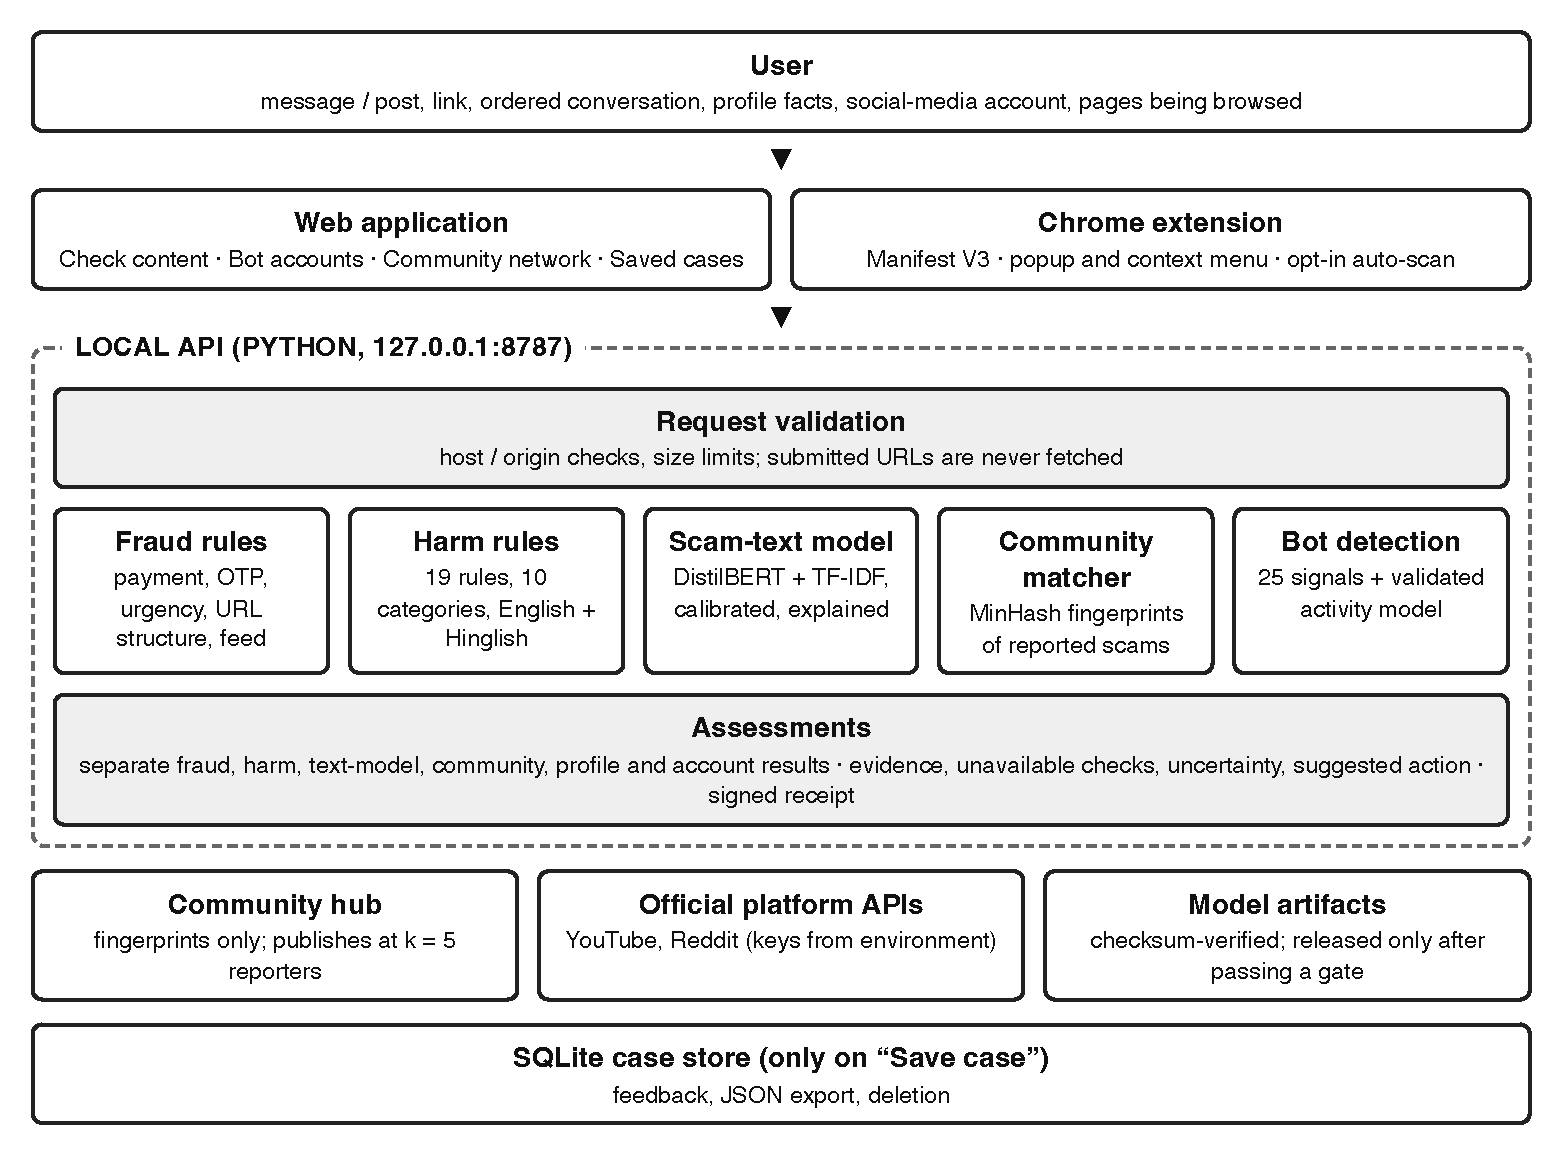
\includegraphics[width=0.8\linewidth]{dia2/block_v2.pdf}
\caption{General block diagram of Sentinel}
\label{fig:block}
\end{figure}

\noindent\textbf{Organization of the report.} Chapter 2 reviews existing work, Chapter 3 describes the design, Chapter 4 the plan and test setup, Chapter 5 the results, Chapter 6 the conclusion and Chapter 7 the references.

\titleformat{\chapter}[display]{\bfseries\centering}{\huge Chapter \thechapter}{1em}{\Huge #1}

\newgeometry{top=3cm, bottom=2.2cm, left=3cm, right=2cm, headsep=1.2cm, footskip=1cm, headheight=0.3cm, textheight=24.5cm, textwidth=16cm}
\onehalfspacing

\pagestyle{fancy}
\fancyhf{}
\renewcommand{\headrulewidth}{0pt}
\lhead{Chapter 2}
\rhead{Literature Survey}
\cfoot{\thepage}
\chapter{Literature Survey}

\section{Survey of Existing Systems}
\noindent We studied four groups of work: fake-profile and bot detection, cyberbullying and hate-speech detection, SMS scam datasets, and phishing-URL tools.

\subsection{Research Papers}
\begin{itemize}
\item \textbf{Fake profiles \cite{lit1,lit2,lit3}:} these papers use profile details, posts, images and even login behaviour to find fake accounts. Aditya and Mohanty \cite{lit2} report 93.5\% accuracy, but need platform data that a normal user cannot see.
\item \textbf{Cyberbullying \cite{lit4,lit5}:} Atif et al. \cite{lit4} detect bullying in Roman Urdu tweets (97\% F1); Ibrahim et al. \cite{lit5} handle overlapping hate-speech classes. Neither checks links or accounts.
\item \textbf{Social bots \cite{cresci2015,cresci2017,yang2020}:} Cresci et al. built datasets of fake followers and human-like ``social spambots'' that are hard to spot. Yang et al. showed that a bot detector trained on one dataset often fails on another, which is why Sentinel tests its bot models on whole datasets they have never seen.
\item \textbf{Datasets \cite{phiusiil,cad,smsdata}:} PhiUSIIL (235,795 URLs), CAD (Reddit abuse with context) and an SMS phishing dataset (5,971 messages labelled ham, spam or smishing) are used in Sentinel's studies.
\end{itemize}

\subsection{Real-Time Systems}
\noindent \textbf{PhishTank} \cite{phishtank} and \textbf{Google Safe Browsing} \cite{safebrowsing} keep lists of known bad URLs. They are accurate for known links, but cannot judge a new link, do not explain their answer and do not look at message text, harmful language or accounts. \textbf{Platform moderation} acts only after users report, and rarely explains itself.

\subsection{Summary of the Survey}
\begin{footnotesize}
\renewcommand{\arraystretch}{1.15}
\begin{longtable}{|>{\raggedright\arraybackslash}p{3.4cm}|>{\raggedright\arraybackslash}p{4.1cm}|>{\raggedright\arraybackslash}p{3.2cm}|>{\raggedright\arraybackslash}p{3.3cm}|}
\caption{Summary of the literature survey}\label{tab:lit}\\
\hline
\textbf{Work} & \textbf{Method} & \textbf{Result} & \textbf{Drawback} \\ \hline
\endfirsthead
\hline
\textbf{Work} & \textbf{Method} & \textbf{Result} & \textbf{Drawback} \\ \hline
\endhead
Bhambulkar et al. \cite{lit1} & Review of ML/DL fake-profile methods & Lists useful profile features & Profiles only; no links or messages \\ \hline
Aditya and Mohanty \cite{lit2} & Word2Vec + CNN on posts, media, logins & 93.5\% accuracy & Needs platform-side data \\ \hline
Habib et al. \cite{lit3} & Survey of fake-profile techniques & Overview for future work & No new experiments \\ \hline
Atif et al. \cite{lit4} & GRU for Roman Urdu bullying & 97\% F1 & One language; no phishing \\ \hline
Ibrahim et al. \cite{lit5} & Neutrosophic MLP for hate speech & Better on mixed classes & Text only \\ \hline
Cresci et al. \cite{cresci2015,cresci2017} & Fake-follower and spambot datasets & Human-like bots are hard to spot & Twitter only, up to 2017 \\ \hline
Yang et al. \cite{yang2020} & Cross-dataset bot testing & One-dataset models generalise poorly & Needs platform data \\ \hline
PhiUSIIL \cite{phiusiil}, CAD \cite{cad}, SMS set \cite{smsdata} & Public datasets & Benchmarks for URLs, abuse, SMS & Each covers one threat \\ \hline
PhishTank, Safe Browsing & Lists of known bad URLs & Accurate for known links & No new links; no reasons \\ \hline
\end{longtable}
\end{footnotesize}

\section{Limitations of Existing Systems and Research Gap}
\begin{enumerate}
\item They handle \textbf{one threat at a time}, though one post often mixes a scam message, a link and a fake account.
\item They need \textbf{platform data} that ordinary users cannot see.
\item They give a \textbf{verdict without a reason} and do not say what they could not check.
\item Their \textbf{test results are often optimistic}: models that score highly on one dataset fail on new data.
\item They miss \textbf{Hinglish and disguised words}, and cloud tools send private messages to a server.
\end{enumerate}

\noindent\textbf{Research gap.} There is no simple tool that runs on the user's own computer, checks scam messages, links, harmful language and accounts together, explains every result, lets users warn each other without sharing text, and uses a learned model only after a fair test on unseen data.

\section{Scope of the Proposed System}
\noindent\textbf{In scope:} a local web app and Chrome extension (with opt-in auto-scan); fraud rules; English and Hinglish harm rules; a learned scam-text model; a community scam network with a simulation; bot detection from official APIs or user data; saving cases; and research pipelines for URL, SMS and bot models.\\

\noindent\textbf{Out of scope:} automatic blocking, scraping, opening suspicious links, identity verification, deepfakes, mobile apps and paid cloud services.

\begin{table}[H]
\centering
\footnotesize
\renewcommand{\arraystretch}{1.15}
\caption{Feature comparison of Sentinel with existing systems (``--'': not described)}
\label{tab:features}
\begin{tabular}{|>{\raggedright\arraybackslash}p{4.2cm}|c|c|c|c|c|}
\hline
\textbf{Feature} & \textbf{Sentinel} & \textbf{[2]} & \textbf{[4]} & \textbf{PhishTank} & \textbf{Safe Browsing} \\ \hline
Phishing link check & Yes & No & No & Yes (list) & Yes (list) \\ \hline
Message text check & Yes & No & -- & No & No \\ \hline
Harmful-language check & Yes & No & Yes & No & No \\ \hline
Fake / bot account check & Yes & Yes & Partly & No & No \\ \hline
Hinglish or code-mixed text & Yes & No & Roman Urdu & No & No \\ \hline
Community warnings & Yes & No & No & URLs & No \\ \hline
Works on user-visible data only & Yes & No & Partly & Yes & Yes \\ \hline
Explains evidence and missing checks & Yes & No & No & No & No \\ \hline
Runs locally, no cloud & Yes & No & -- & Feed download & No \\ \hline
\end{tabular}
\end{table}

\titleformat{\chapter}[display]{\bfseries\centering}{\huge Chapter \thechapter}{1em}{\Huge #1}
\newgeometry{top=3cm, bottom=2.2cm, left=3cm, right=2cm, headsep=1.2cm, footskip=1cm, headheight=0.3cm, textheight=24.5cm, textwidth=16cm}
\onehalfspacing
\pagestyle{fancy}
\fancyhf{}
\renewcommand{\headrulewidth}{0pt}
\lhead{Chapter 3}
\rhead{Proposed System}
\cfoot{\thepage}
\chapter{Proposed System}

\section{Detailed Explanation of the Proposed System}
\noindent Sentinel is built in five layers (Figure~\ref{fig:arch}):
\begin{enumerate}
\item \textbf{Input:} the web app and the Chrome extension collect a message, link, chat, profile or account, or read the visible text of a page when auto-scan is on.
\item \textbf{Preprocessing:} the server checks that the request is valid and safe. Links are read as text only and never opened.
\item \textbf{Threat detection:} separate checkers look at the input: fraud rules, harm rules, the scam-text model, the community matcher, profile checks and bot detection.
\item \textbf{Analysis:} each checker gives its own level (for example High, Review or Low concern) with its evidence. Results are never merged into one score.
\item \textbf{Output:} the results appear as cards in the web app, in the extension popup, or as markers on the web page. The user can save a case.
\end{enumerate}

\noindent\textbf{Working principle.} Every result says what was \emph{observed}, what \emph{could not be checked}, and what to do next, so ``nothing found'' is never shown as ``safe''. A learned model is used only if its files pass a checksum test and the model passed its release test; if it fails at run time, its card says ``unavailable'' and the rules still work.

\begin{figure}[H]
\centering
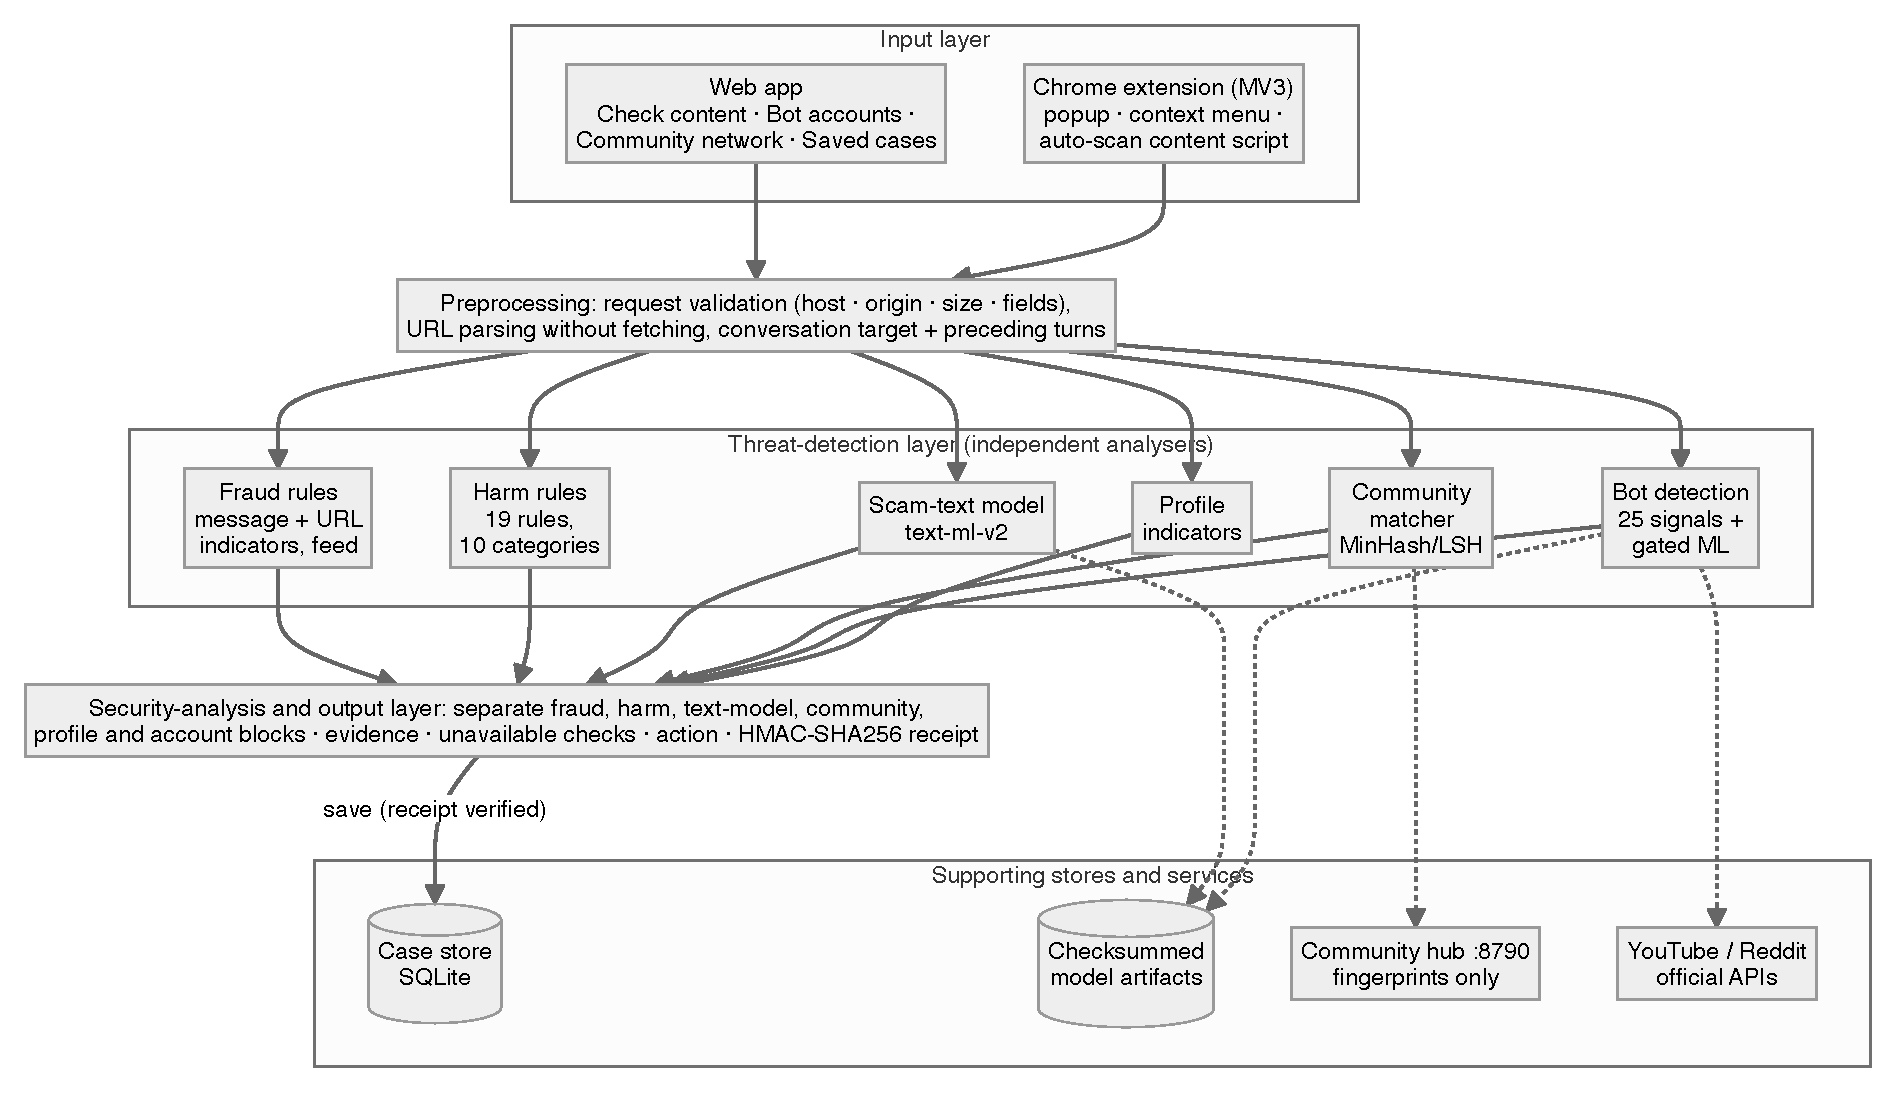
\includegraphics[width=0.95\linewidth]{dia2/arch_v2.pdf}
\caption{Layered architecture of Sentinel}
\label{fig:arch}
\end{figure}

\subsection{Module-wise Explanation}
\begin{enumerate}[label=\textbf{M\arabic*}, leftmargin=1.1cm]
\item \textbf{Web app:} four pages: \emph{Check content}, \emph{Bot accounts}, \emph{Community network} and \emph{Saved cases}. Results are shown as cards; a high-risk harm card moves to the top.
\item \textbf{Chrome extension:} a popup and right-click menu for quick checks, plus \emph{auto-scan}. When the user turns auto-scan on for a site, the extension reads the text visible on screen, sends it in small batches to the local server and marks risky messages without changing the page. It can also read text and QR codes inside images on that site, using OCR that runs inside the extension. If the server is off, it waits and retries; it never shows anything as ``safe''.
\item \textbf{Local server (\texttt{server.py}):} a Python web server that only listens on the user's own computer. It rejects requests from other websites, limits request size and adds browser security headers.
\item \textbf{Fraud rules:} look for requests for money or fees, passwords or OTPs, and urgency, and for suspicious links (an IP address instead of a name, ``@'' in the address, punycode, very long links). An optional list of known phishing links can be loaded.
\item \textbf{Harm rules:} 19 rules in 10 groups, such as threats, self-harm, sextortion, blackmail, stalking, hate and harassment, in English and Hinglish. They first undo disguises (\texttt{1d10t}$\to$idiot, \texttt{k.y.s}$\to$kys) and then check context: idioms (``this movie killed it'') are ignored, ``I would never hurt you'' is not a threat, and quoted insults go to human review. Self-harm messages get helpline numbers (Tele-MANAS 14416) \cite{telemanas}.
\item \textbf{Scam-text model (text-ml-v2):} a DistilBERT model and a TF-IDF model, averaged. It labels a message as genuine, spam or smishing, gives a probability, and highlights the words that raised the score.
\item \textbf{Batch scan:} the auto-scan endpoint. It runs all checks on up to 40 page items at once and gives each a severity: high, review or none.
\item \textbf{Community network:} when a user's Sentinel finds a scam, it can (if the user agrees) send only a \emph{fingerprint} of it to a hub. When 5 different users report the same scam, the hub publishes it, and every user is warned, even if their own model missed it. The hub never sees the message text.
\item \textbf{Bot detection:} takes a profile link, an uploaded file or typed details, and gets data only from the official YouTube or Reddit APIs or from the user. It scores 25 signals (posting rhythm, repeated posts, follower ratio and others) and shows which signals mattered. A trained activity model adds a probability for X accounts.
\item \textbf{Profile checks:} simple flags such as very many posts per day or following far more accounts than follow back.
\item \textbf{Receipts and case store:} each result carries a signed receipt (HMAC). A case can be saved only with a valid receipt, so the saved result is exactly what the user saw. Cases are stored in a local SQLite file and can be exported or deleted.
\item \textbf{Research pipeline:} command-line tools to download datasets (checked by SHA-256), split them fairly, train, calibrate and test models once on held-out data.
\end{enumerate}

\section{System Analysis}
\subsection{Functional Requirements}
\begin{enumerate}[label=FR\arabic*:, leftmargin=1.3cm]
\item Accept a message, link, chat, profile details or account, alone or together.
\item Reject empty, too large or invalid requests with a clear error.
\item Report fraud, harm, model, community and account results separately, each with evidence, missing checks and an action.
\item Never open a submitted link or scrape a profile.
\item Detect harmful language in English and Hinglish and give advice by urgency.
\item Scan visible page text only on sites the user switched on, and mark risky items.
\item Share only anonymous fingerprints with the hub, and only if the user agrees.
\item Analyse accounts from official APIs, uploads or manual entry; reject unsafe profile links.
\item Save, list, export and delete cases; save only with a valid receipt.
\end{enumerate}

\subsection{Non-Functional Requirements}
\begin{itemize}
\item \textbf{Privacy:} everything runs on the user's computer; nothing is stored unless saved; the hub stores no message text.
\item \textbf{Security:} local-only server, origin checks, size limits, security headers, signed receipts, safe link parsing, rate limits, API keys only from environment variables.
\item \textbf{Explainability:} every result explains its evidence in plain words.
\item \textbf{Performance:} rule checks take milliseconds; the text model takes about 2 ms per message on a laptop CPU.
\item \textbf{Reliability:} a broken model or offline hub shows ``unavailable''; it never breaks the check.
\item \textbf{Portability:} runs on Windows, macOS or Linux with Python and Chrome.
\end{itemize}

\subsection{Software and Hardware Requirements}
\begin{table}[H]
\centering
\small
\renewcommand{\arraystretch}{1.2}
\caption{Software and hardware requirements}
\label{tab:swhw}
\begin{tabular}{|>{\raggedright\arraybackslash}p{3.5cm}|>{\raggedright\arraybackslash}p{11.3cm}|}
\hline
\textbf{Component} & \textbf{Requirement} \\ \hline
Operating system & Windows 10/11, macOS or Linux \\ \hline
Application & Python 3.10+ (rules need only the standard library); SQLite \\ \hline
Models & ONNX Runtime, \texttt{tokenizers}, scikit-learn, NumPy; PyTorch and Transformers only for training \\ \hline
Browser and tests & Google Chrome; Python \texttt{unittest}; Node.js for JavaScript tests \\ \hline
Hardware & Laptop with 16 GiB RAM (AMD Ryzen 7 7435HS or Apple M4) \\ \hline
Network & Not needed for checks; only for the optional YouTube/Reddit APIs and dataset downloads \\ \hline
\end{tabular}
\end{table}

\subsection{Use Case Modelling}
\noindent Figure~\ref{fig:usecase} shows the main actors: the \emph{User}, the \emph{Research team member} and the optional \emph{Phishing feed}. Table~\ref{tab:uc} summarises the main use cases, including those added in this phase.
\begin{figure}[H]
\centering
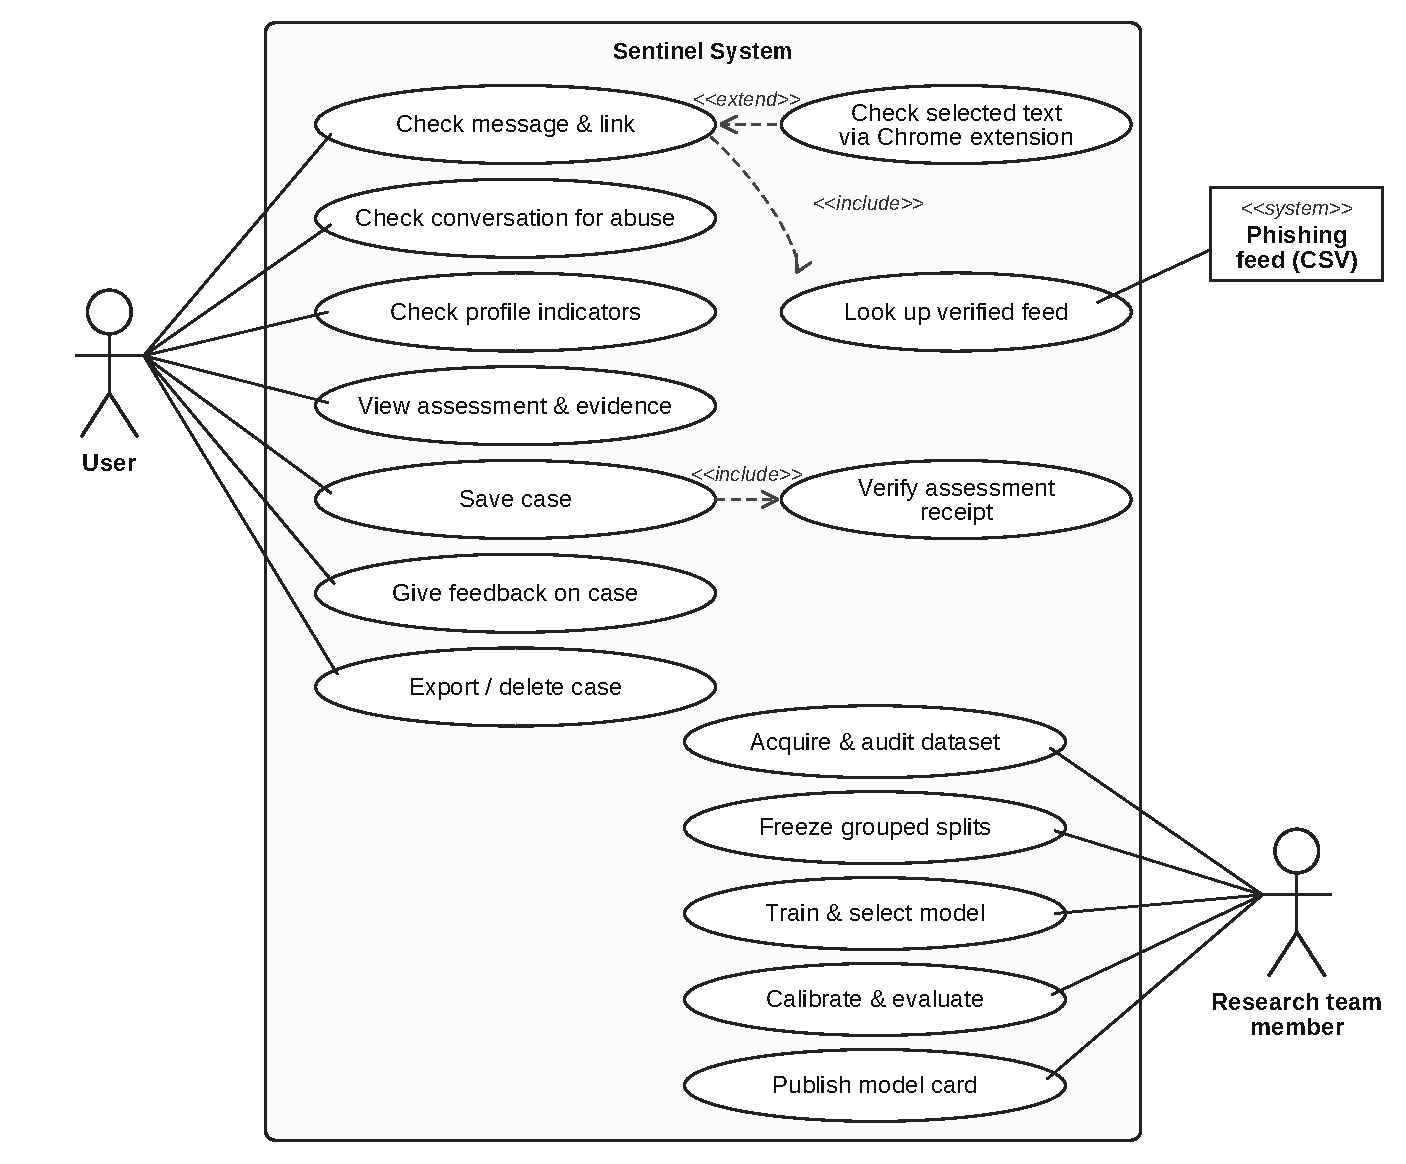
\includegraphics[width=0.82\linewidth]{dia/usecase.pdf}
\caption{Use case diagram (core check)}
\label{fig:usecase}
\end{figure}

\begin{table}[H]
\centering
\footnotesize
\renewcommand{\arraystretch}{1.2}
\caption{Main use cases}
\label{tab:uc}
\begin{tabular}{|l|>{\raggedright\arraybackslash}p{2.6cm}|>{\raggedright\arraybackslash}p{7.2cm}|>{\raggedright\arraybackslash}p{3.3cm}|}
\hline
\textbf{ID} & \textbf{Use case} & \textbf{Main steps} & \textbf{Result} \\ \hline
UC-01 & Check a message and link & Paste content, click \emph{Analyze}; server validates and runs all checkers; result cards appear & Cards with evidence; nothing stored \\ \hline
UC-02 & Save a case & Click \emph{Save}; server checks the receipt (same input, under 15 min) and stores the case & Case listed; can export or delete \\ \hline
UC-03 & Auto-scan a page & Turn auto-scan on for a site; visible text is batched and scanned; risky items are marked & Markers and badge count; page unchanged \\ \hline
UC-04 & Check an account & Enter a link or upload posts; data comes from an official API or the file; 25 signals are scored & Score, confidence and top signals \\ \hline
UC-05 & Train and test a model & Download and verify data, split, train, calibrate, test once & Model card; released only if it passes \\ \hline
\end{tabular}
\end{table}

\section{Proposed System: Analysis, Modelling and Design}
\noindent The activity, sequence, class, ER and data-flow diagrams below describe the core content check; a second sequence diagram shows auto-scan, and the deployment diagram shows all parts.

\subsection{Activity Diagram}
\noindent Figure~\ref{fig:activity} follows one check: the request is checked, the checkers run side by side, and the result is shown and optionally saved.
\begin{figure}[H]
\centering
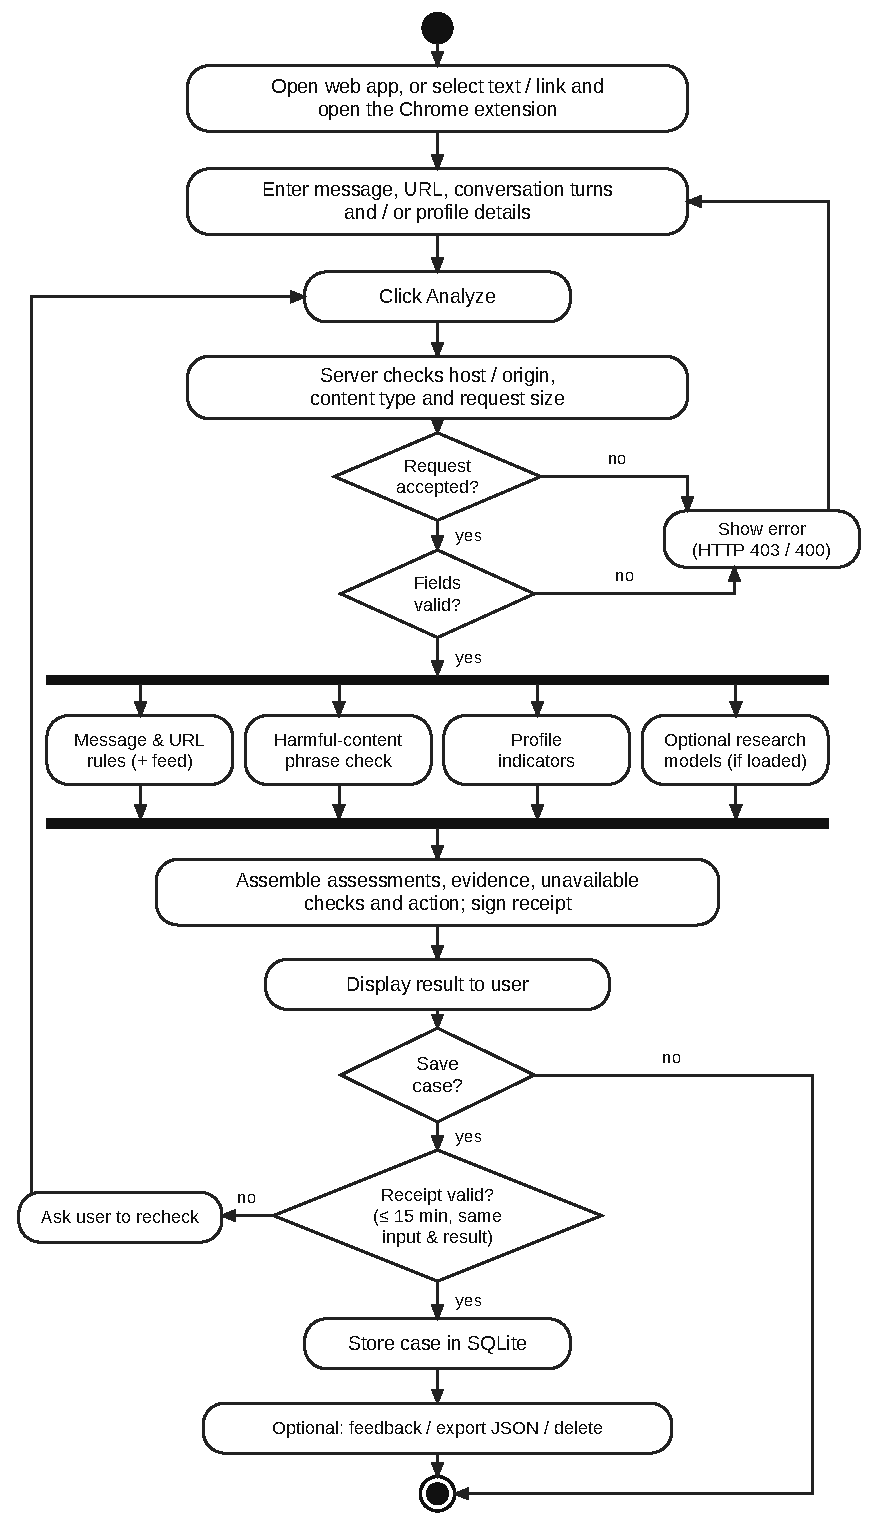
\includegraphics[height=0.62\textheight]{dia/activity.pdf}
\caption{Activity diagram of a Sentinel check}
\label{fig:activity}
\end{figure}

\subsection{Sequence Diagrams}
\noindent Figure~\ref{fig:sequence} shows a check and a save: the server analyses the content and signs a receipt, and later verifies the receipt before saving. Figure~\ref{fig:autoscan} shows auto-scan.
\begin{figure}[H]
\centering
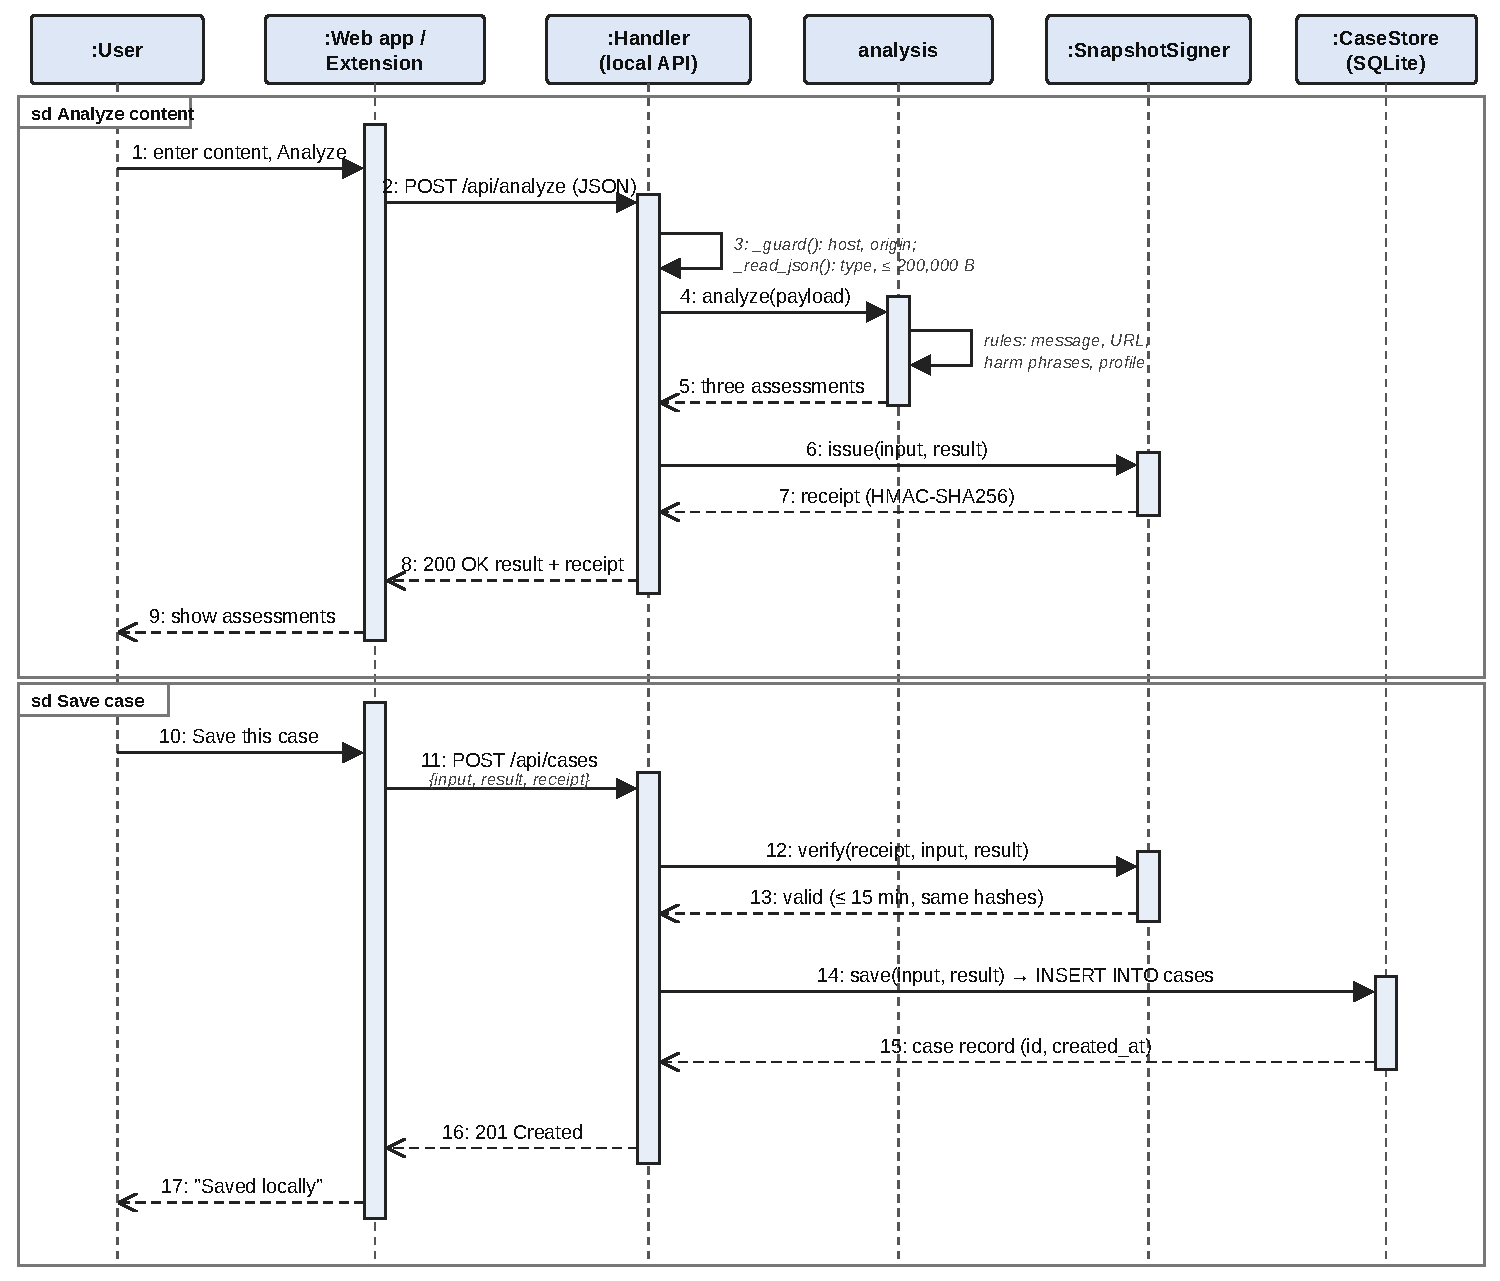
\includegraphics[width=\linewidth]{dia/sequence.pdf}
\caption{Sequence diagram: analysing content and saving a case}
\label{fig:sequence}
\end{figure}
\begin{figure}[H]
\centering
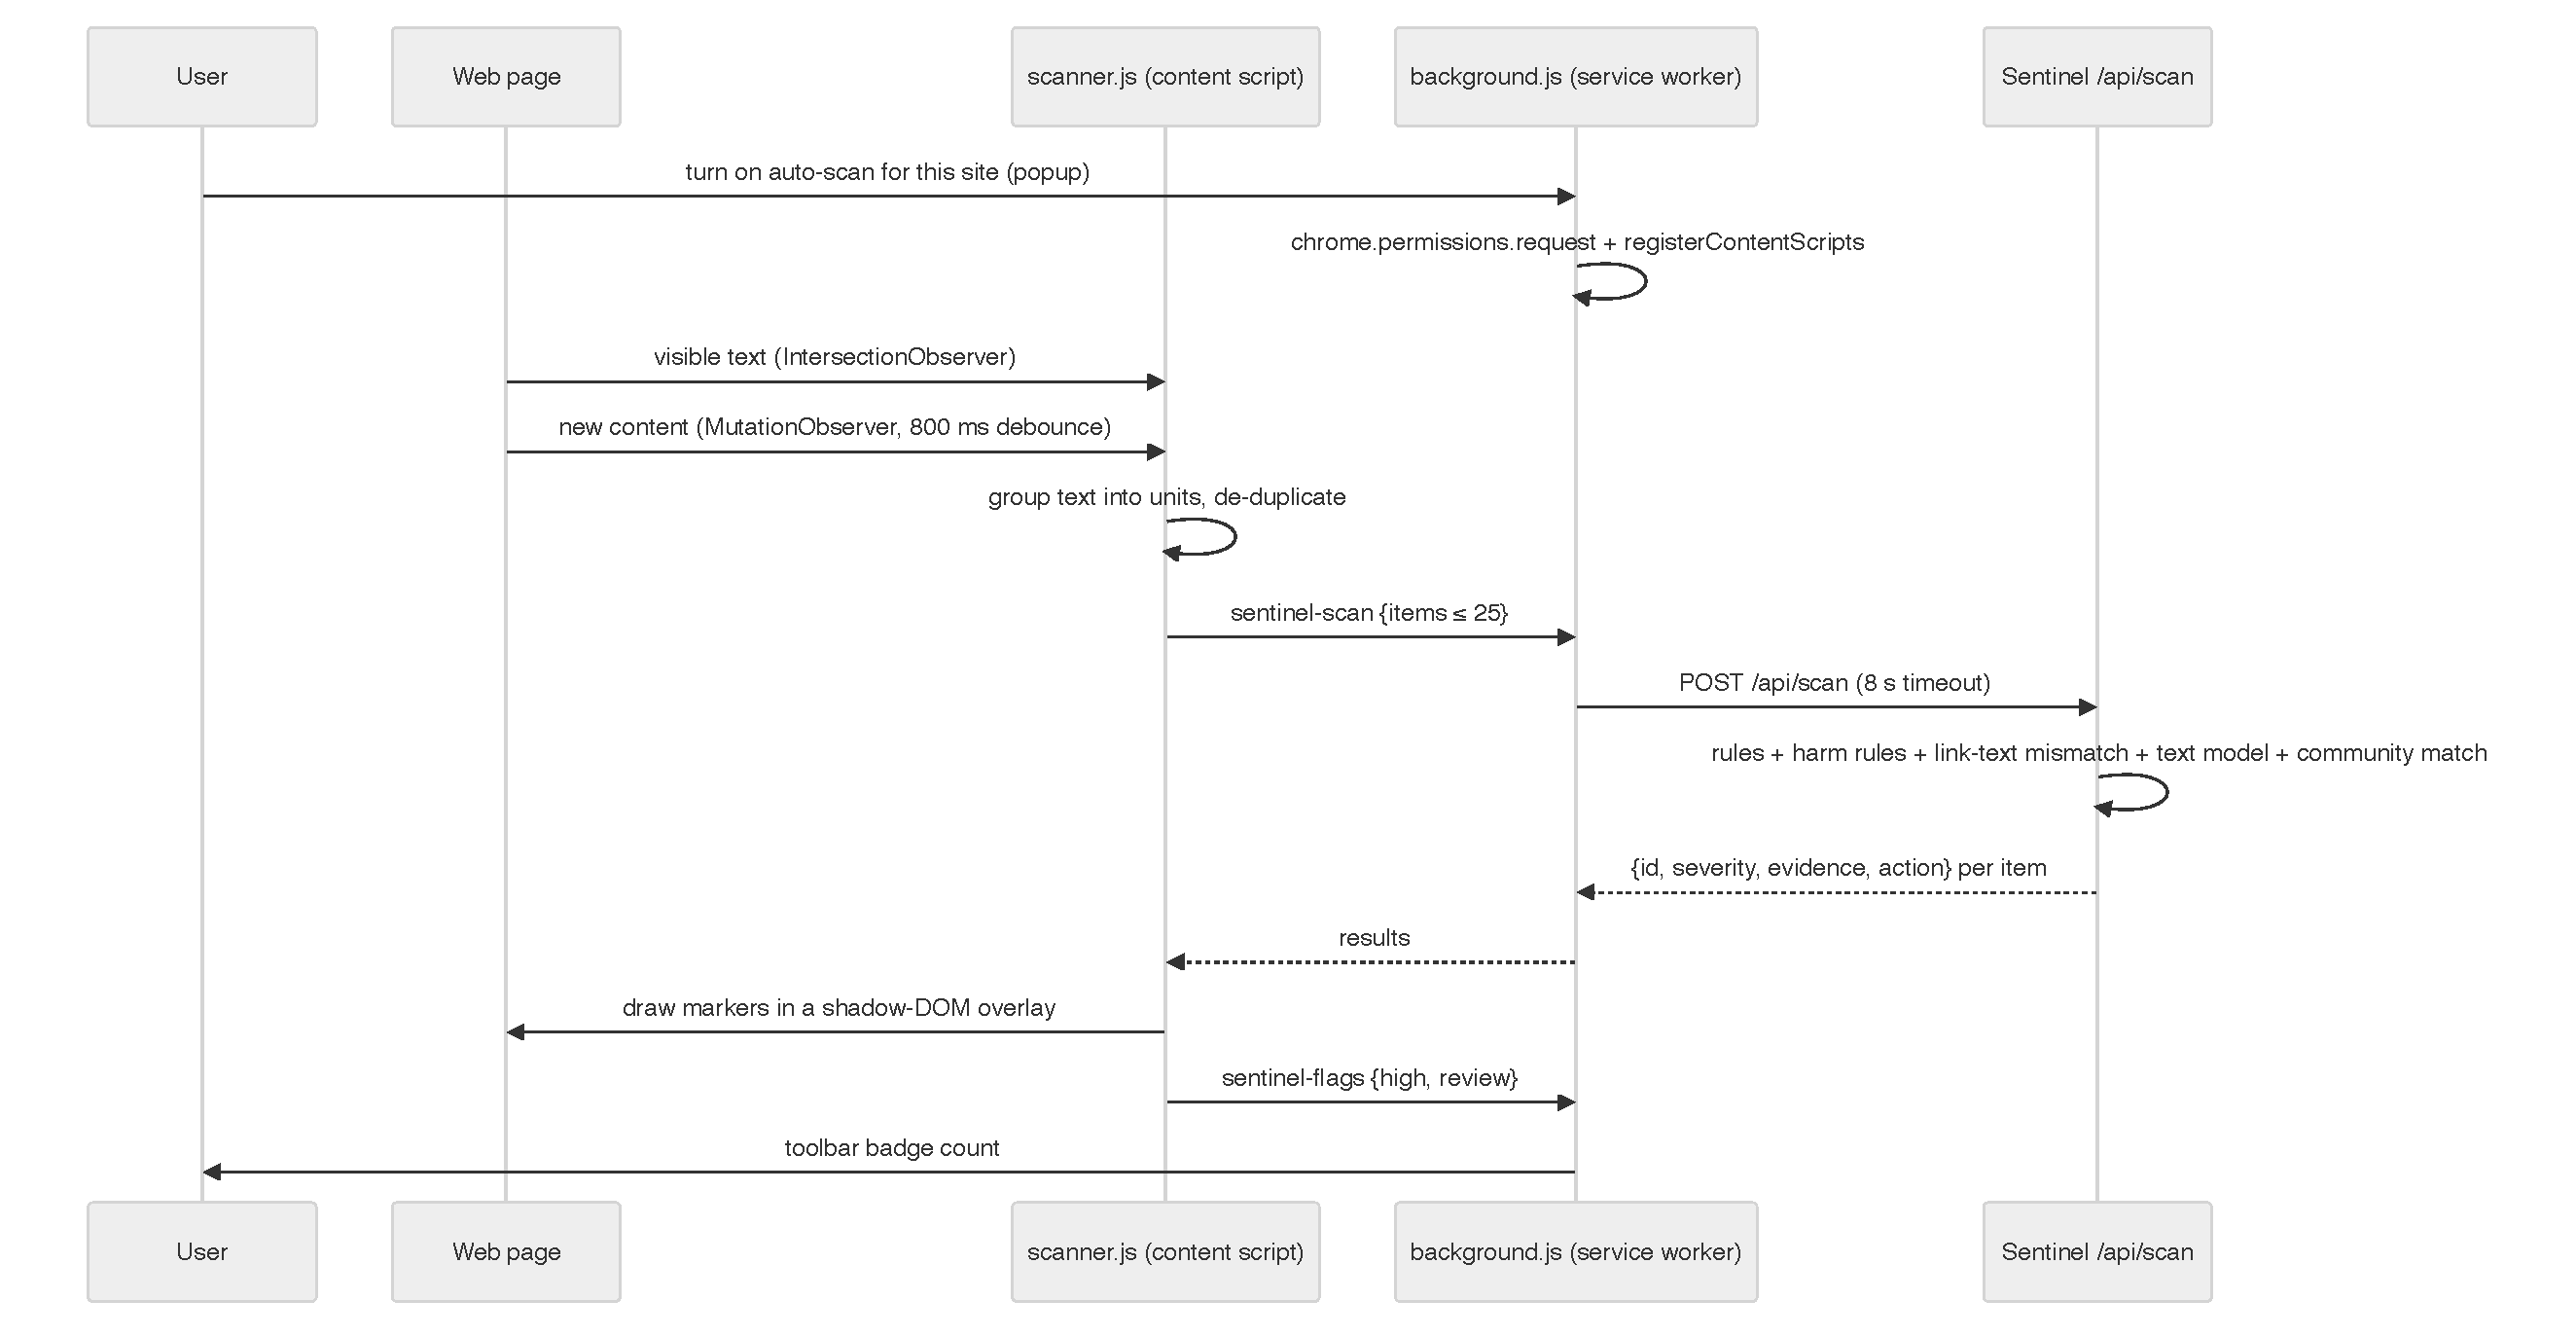
\includegraphics[width=0.92\linewidth]{dia2/autoscan.pdf}
\caption{Sequence diagram: auto-scan of visible page text}
\label{fig:autoscan}
\end{figure}

\subsection{Class Diagram}
\noindent The server creates one case store and one receipt signer, shared by every request handler. The \texttt{analysis} module calls the checkers (Figure~\ref{fig:class}).
\begin{figure}[H]
\centering
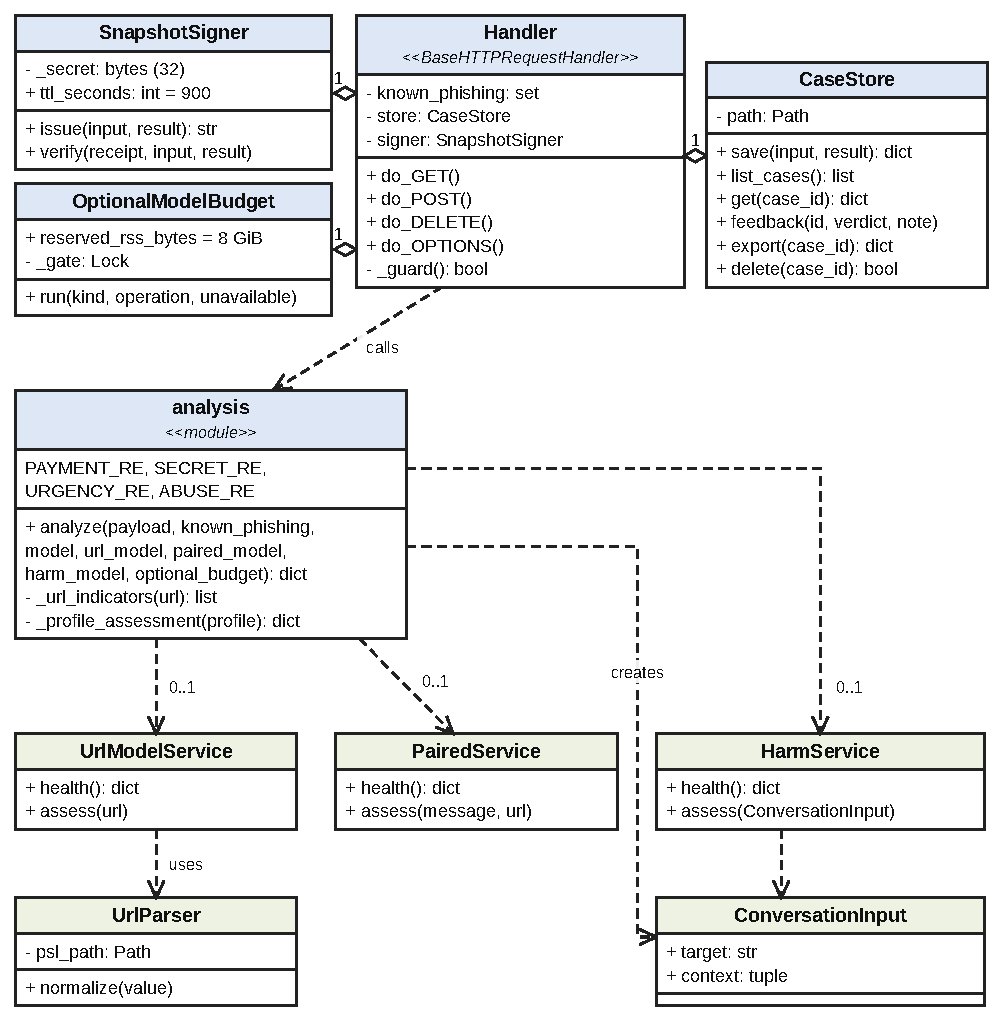
\includegraphics[width=0.78\linewidth]{dia/class.pdf}
\caption{Class diagram of the main application components}
\label{fig:class}
\end{figure}

\subsection{Deployment Diagram}
\noindent Everything runs on the user's computer (Figure~\ref{fig:deploy}): Chrome talks to the Python server, which uses the model files, the case database and, optionally, the community hub and official APIs. Models are trained on a separate research machine and copied over.
\begin{figure}[H]
\centering
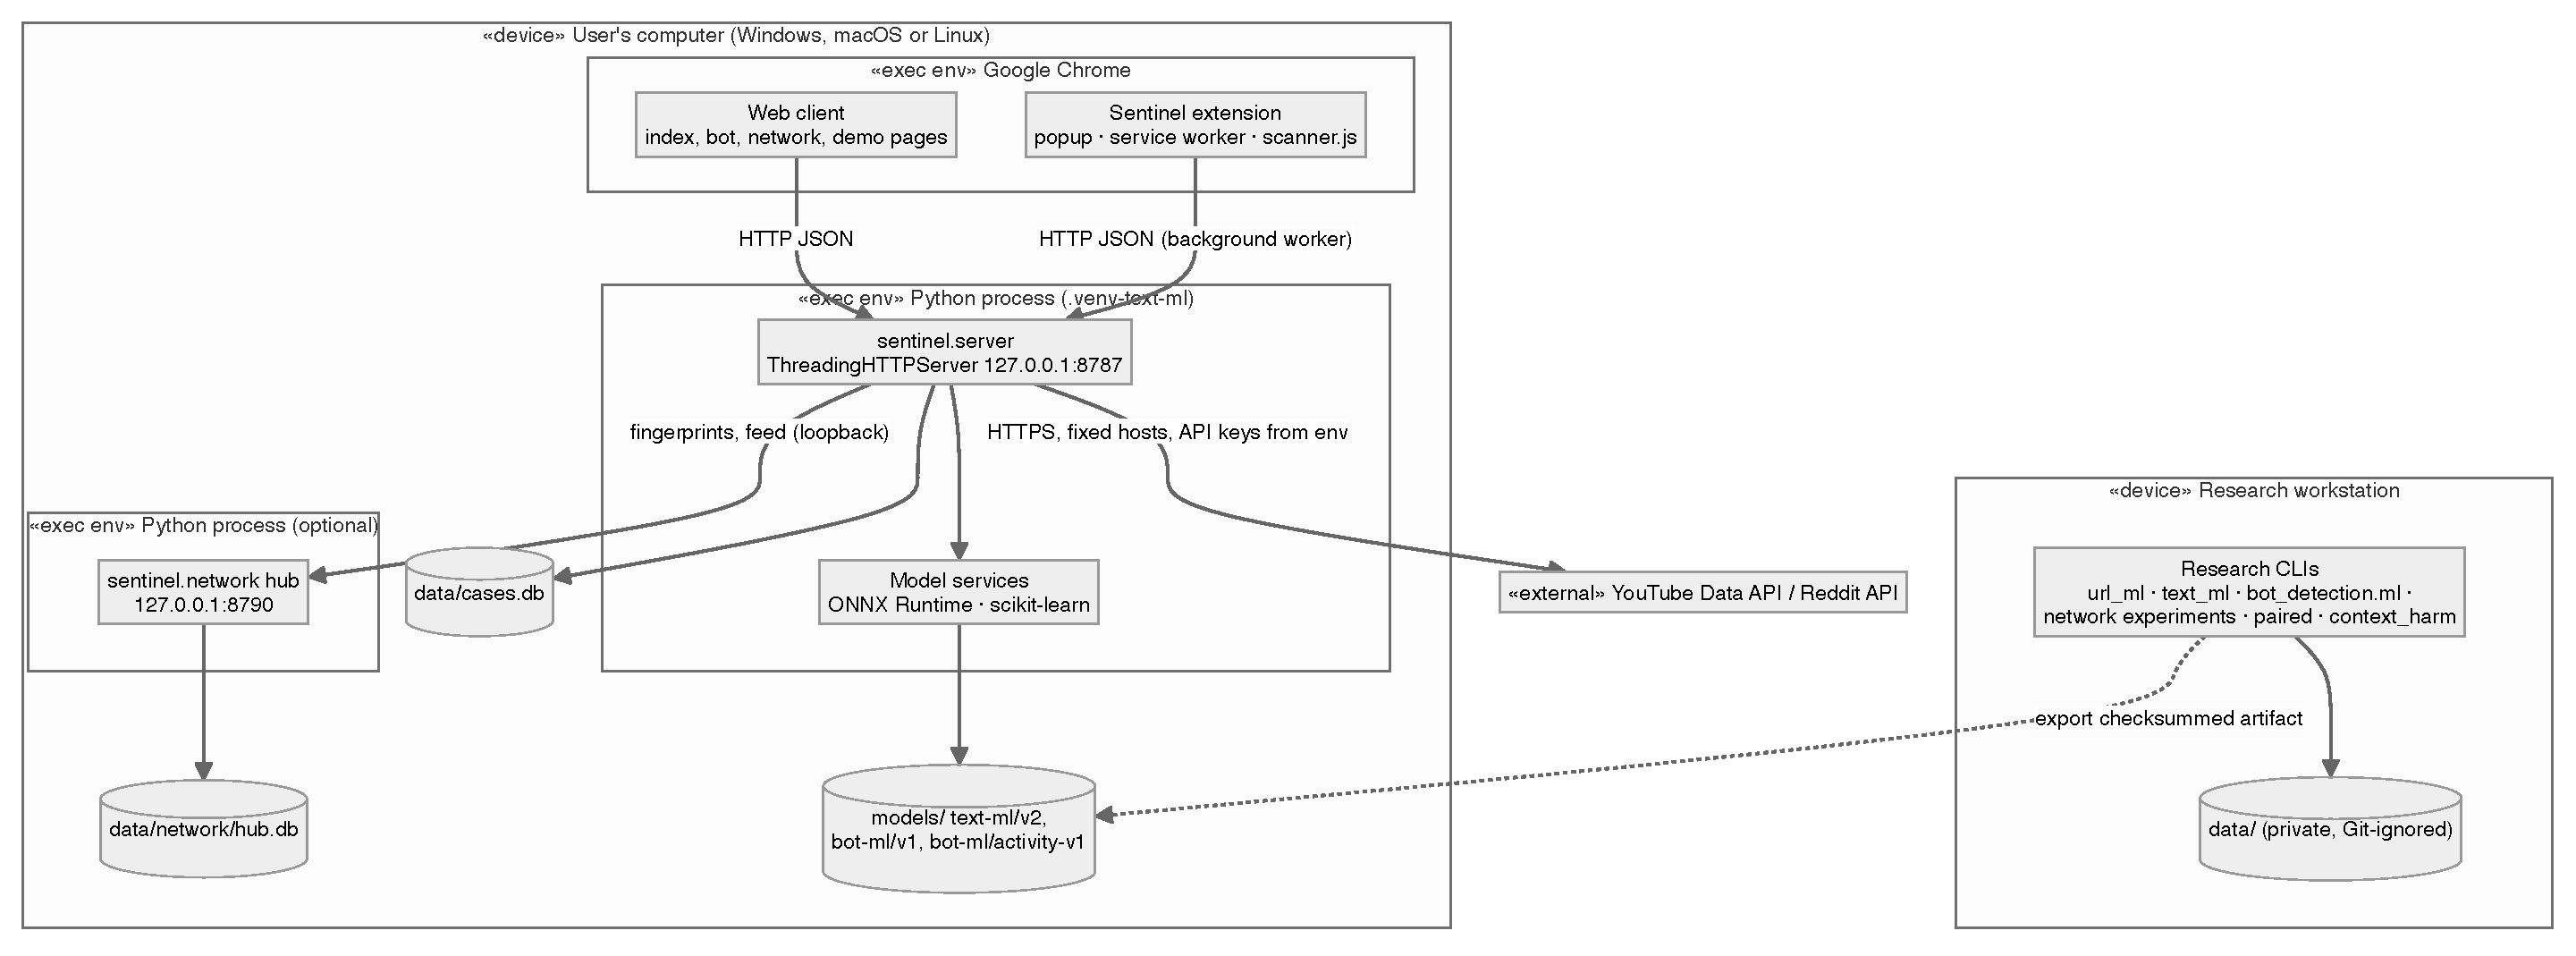
\includegraphics[width=\linewidth]{dia2/deploy_v2.pdf}
\caption{Deployment diagram}
\label{fig:deploy}
\end{figure}

\subsection{ER Diagram and Schema}
\noindent Only saved cases are stored, in one table (Figure~\ref{fig:er}, Table~\ref{tab:schema}). There are no user accounts. The optional hub has its own database of fingerprints, report counts and times, with no message text.
\begin{figure}[H]
\centering
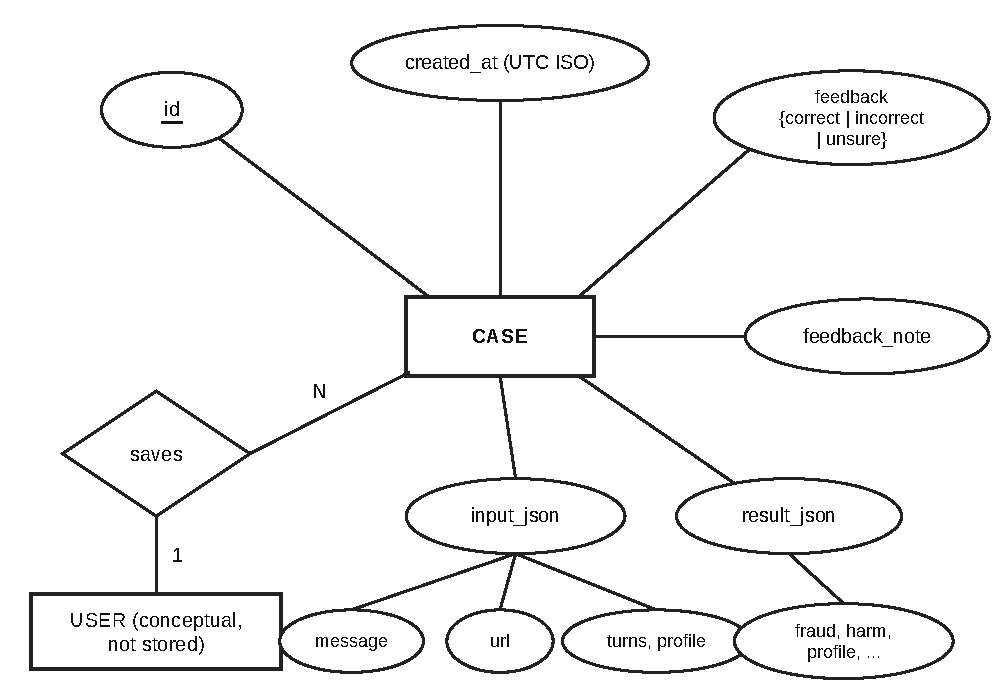
\includegraphics[width=0.62\linewidth]{dia/er.pdf}
\caption{ER diagram of the case store}
\label{fig:er}
\end{figure}
\begin{table}[H]
\centering
\footnotesize
\renewcommand{\arraystretch}{1.15}
\caption{Schema of the \texttt{cases} table}
\label{tab:schema}
\begin{tabular}{|l|l|>{\raggedright\arraybackslash}p{9cm}|}
\hline
\textbf{Column} & \textbf{Type} & \textbf{Meaning} \\ \hline
id & TEXT (key) & Random case ID \\ \hline
created\_at & TEXT & Time saved (UTC) \\ \hline
input\_json & TEXT & What the user checked \\ \hline
result\_json & TEXT & The exact result the user saw \\ \hline
feedback, feedback\_note & TEXT & Optional: correct, incorrect or unsure, with a note \\ \hline
\end{tabular}
\end{table}

\subsection{Data Flow Diagrams}
\noindent At Level 0 (Figure~\ref{fig:dfd0}) Sentinel exchanges content and results with the user, gets known phishing links from a feed and data from public datasets. Level 1 (Figure~\ref{fig:dfd1}) splits it into capturing input, analysing content, managing cases and training models.
\begin{figure}[H]
\centering
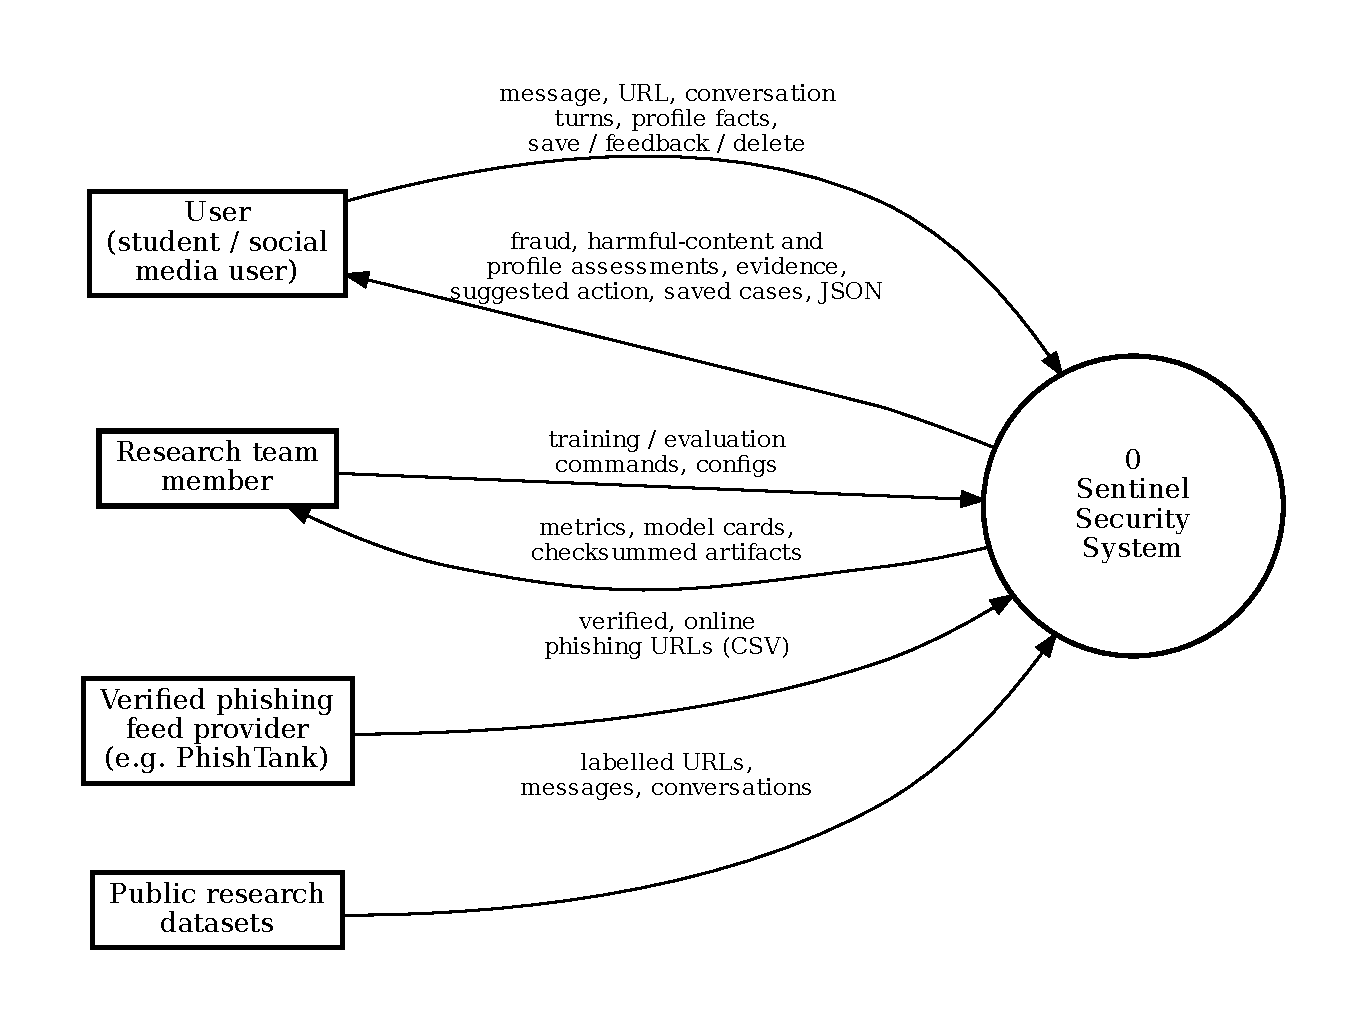
\includegraphics[width=0.72\linewidth]{dia/dfd0.pdf}
\caption{DFD Level 0 (context diagram)}
\label{fig:dfd0}
\end{figure}
\begin{figure}[H]
\centering
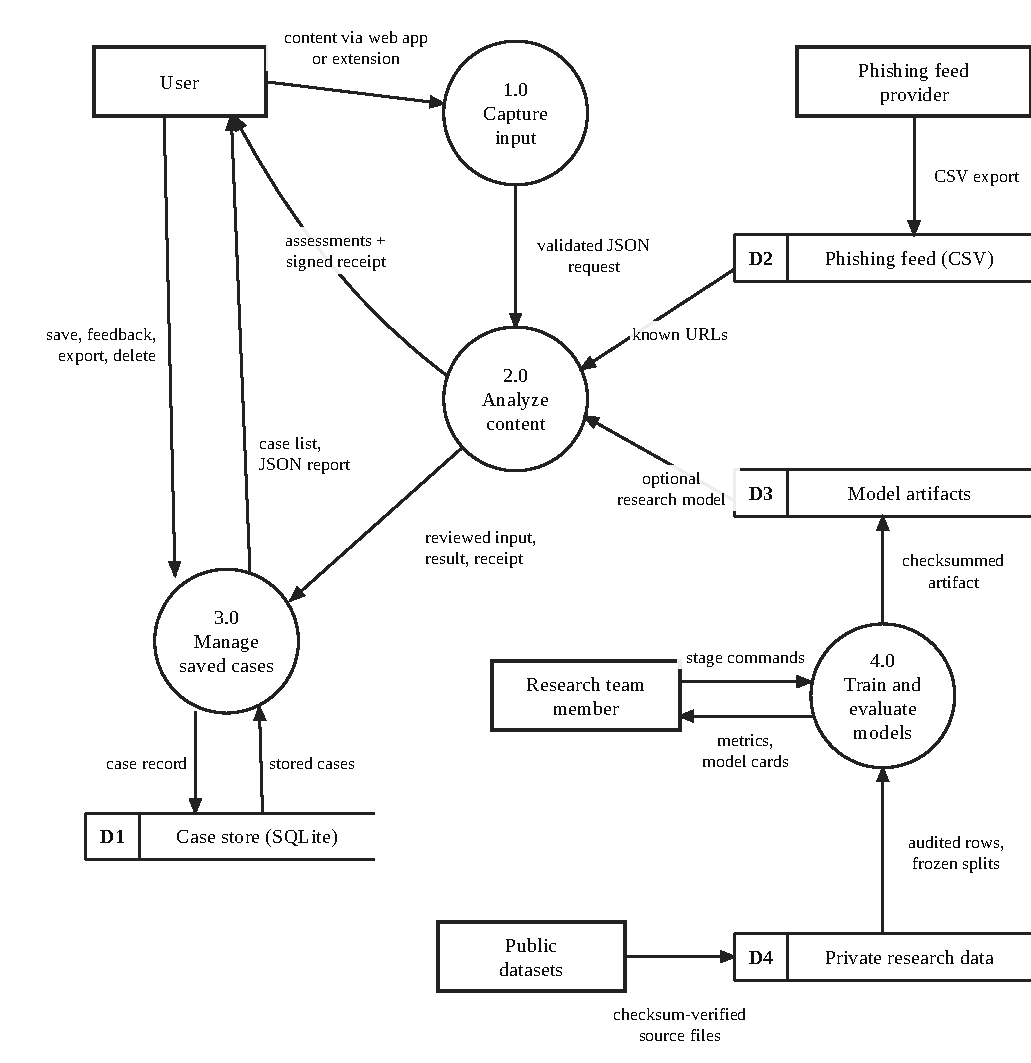
\includegraphics[width=0.78\linewidth]{dia/dfd1.pdf}
\caption{DFD Level 1}
\label{fig:dfd1}
\end{figure}

\subsection{Algorithms and Methodology}\label{sec:algos}
\noindent\textbf{1. Fraud level.} If the link is on the known-phishing list, or the message asks for money or a password \emph{and} the link looks suspicious, the level is \emph{High}. Any other evidence gives \emph{Review}; otherwise \emph{Low observed concern}.\\

\noindent\textbf{2. Harmful language} (Algorithm~\ref{alg:harm}).
\begin{algorithm}[H]
\caption{Harmful-language check}\label{alg:harm}
\begin{algorithmic}[1]
\State clean the text: undo look-alike letters, dotted letters, number-for-letter tricks and stretched letters
\ForAll{each of the 19 rules}
  \State skip matches inside known idioms
  \State if a negation (``never'', ``not'') comes just before: lower the level
  \State if the text is quoted or reported: lower \emph{High} to \emph{Review} (never for self-harm risk)
\EndFor
\State level $\gets$ highest level found; advice $\gets$ advice of the most urgent category
\end{algorithmic}
\end{algorithm}

\noindent\textbf{3. Scam-text model.} DistilBERT's scores are calibrated with a temperature $T=1.29$ and averaged with the TF-IDF model's probabilities $\mathbf{p}^{\mathrm{L}}$:
\begin{equation}
\mathbf{p}=\tfrac12\big(\mathrm{softmax}(\mathbf{z}/T)+\mathbf{p}^{\mathrm{L}}\big),\qquad s=p_{\mathrm{spam}}+p_{\mathrm{smishing}},\qquad \text{warn if } s\ge0.611 .
\end{equation}
The threshold 0.611 was chosen on separate calibration data so that at most 1\% of genuine messages are flagged. To explain a warning, each word is removed in turn and the drop in the score is measured; the biggest drops are shown.\\

\noindent\textbf{4. Community fingerprints.} A message is cut into 3-word pieces, and 64 hash functions give a MinHash fingerprint. Two messages with similarity $J$ share at least one of the 32 fingerprint ``bands'' with probability
\begin{equation}
P(J)=1-\big(1-J^{2}\big)^{32},
\end{equation}
which is 99.7\% at $J=0.41$, so reworded scams still match \cite{mmds}. The hub publishes a scam only after 5 different reporters, gives new users half weight for 24 hours, and removes a campaign if enough users dispute it (Figure~\ref{fig:network}).
\begin{figure}[H]
\centering
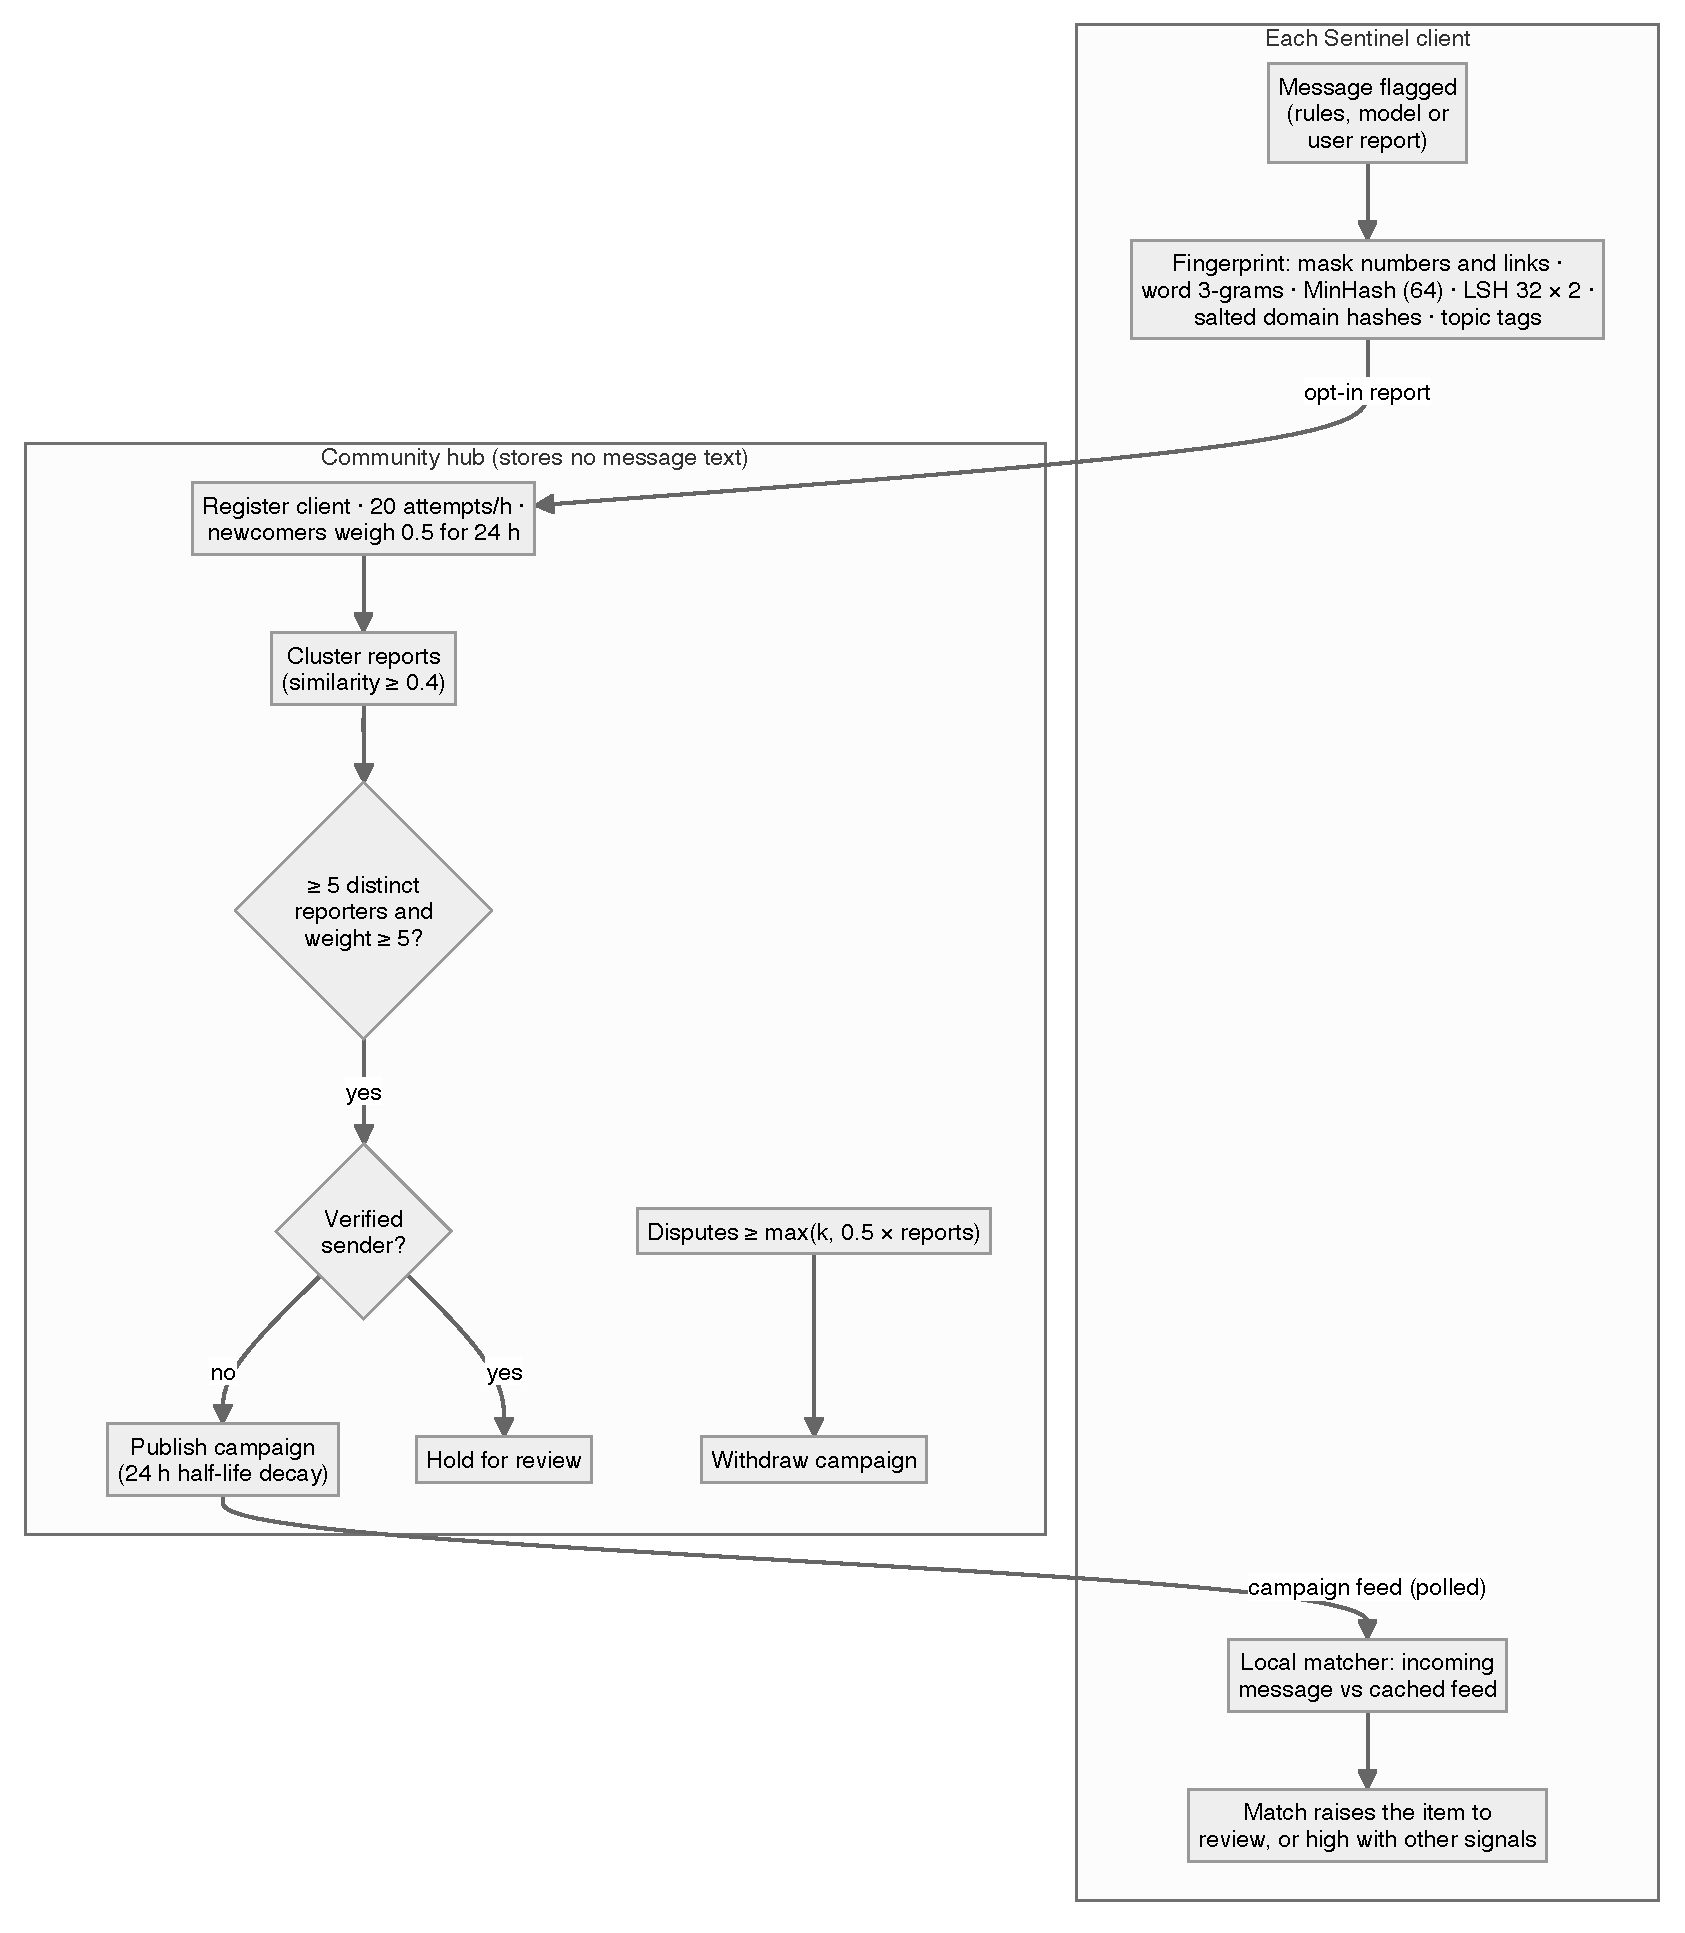
\includegraphics[width=0.55\linewidth]{dia2/network.pdf}
\caption{Community scam network: fingerprinting, publishing and local matching}
\label{fig:network}
\end{figure}

\noindent\textbf{5. Bot score.} Each of the 25 signals gives a suspicion $s_i$ between 0 and 1 and has a weight $w_i$. Only signals with data ($A$) are used:
\begin{equation}
\text{score}=100\cdot\frac{\sum_{i\in A} w_i s_i}{\sum_{i\in A} w_i}.
\end{equation}
If too little data is available (under 25\% of the total weight, or fewer than 4 signals), the score is not shown. For example, bots that post on a timer have almost equal gaps between posts. The trained models use gradient boosting \cite{sklearn} with calibrated probabilities \cite{zadrozny} (Figure~\ref{fig:bot}).
\begin{figure}[H]
\centering
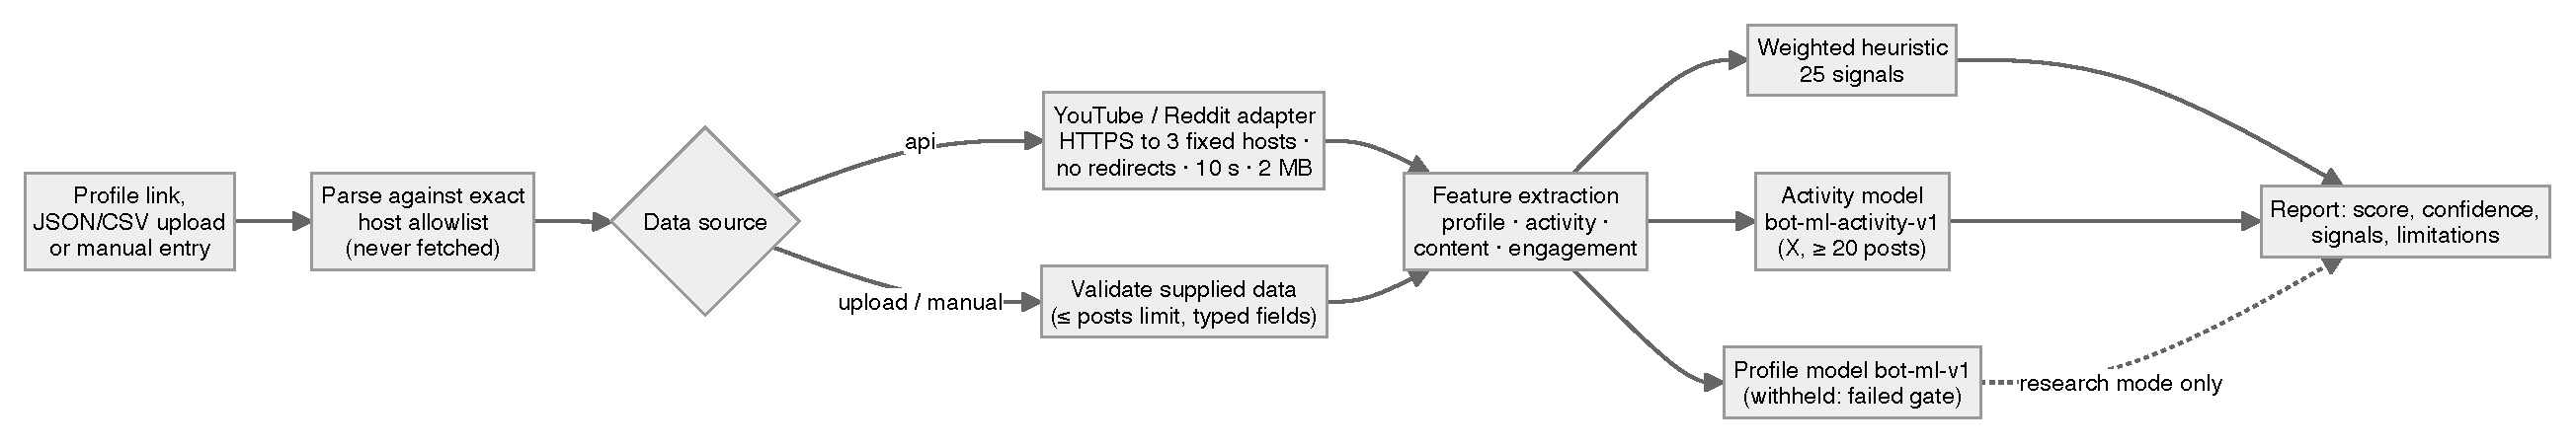
\includegraphics[width=\linewidth]{dia2/bot.pdf}
\caption{Bot-account detection pipeline}
\label{fig:bot}
\end{figure}

\noindent\textbf{6. URL models (research only).} The URL text is split into 3--5 character pieces, turned into TF-IDF features and classified with logistic regression. Data is split by website so that the same site is never in both training and test data.

\subsection{UI/UX Design}
\noindent The design follows four ideas: plain language, separate results for each threat, honesty about limits, and no hidden storage. The check page puts the input on the left and the result cards on the right (Figure~\ref{fig:ui-form}a). Each card shows a level with a text label (not just colour), the evidence, what could not be checked and a next step. The extension popup shows the same cards in a narrow layout (Figure~\ref{fig:ui-form}b; this screenshot is older than the auto-scan switch at the top). The Bot accounts and Community network pages are shown in Figure~\ref{fig:ui-more}.
\begin{figure}[H]
\centering
\begin{minipage}[b]{0.66\linewidth}\centering
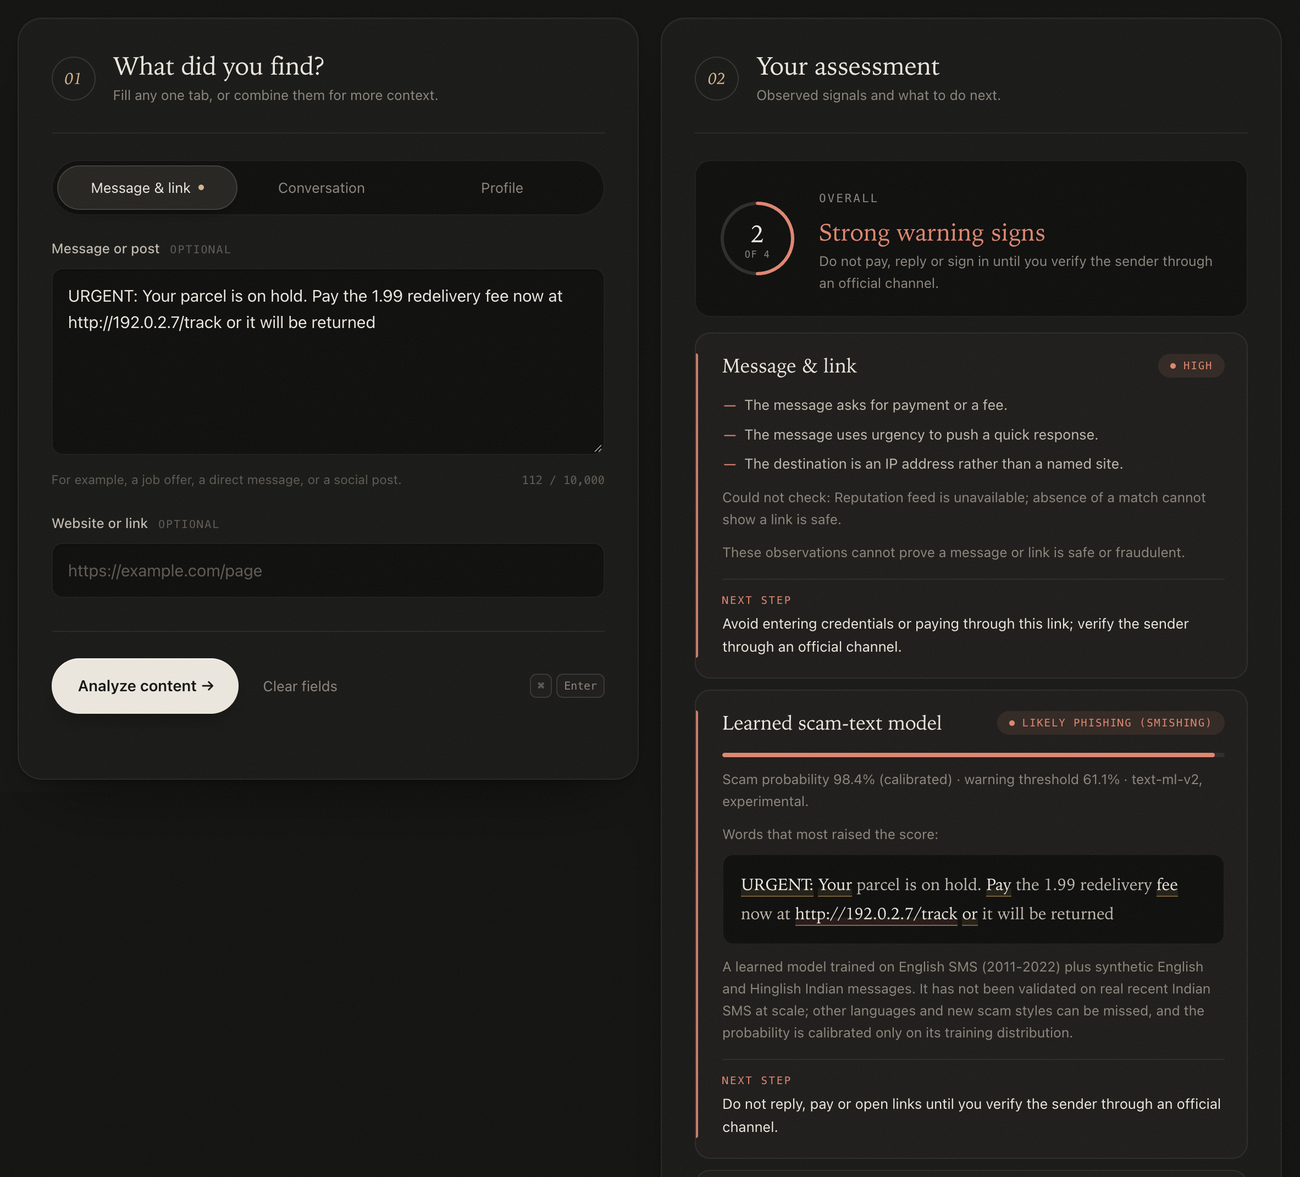
\includegraphics[width=\linewidth]{shots2/check_scam.png}\\[1pt]{\small (a) Check page with a parcel-fee scam}
\end{minipage}\hfill
\begin{minipage}[b]{0.29\linewidth}\centering
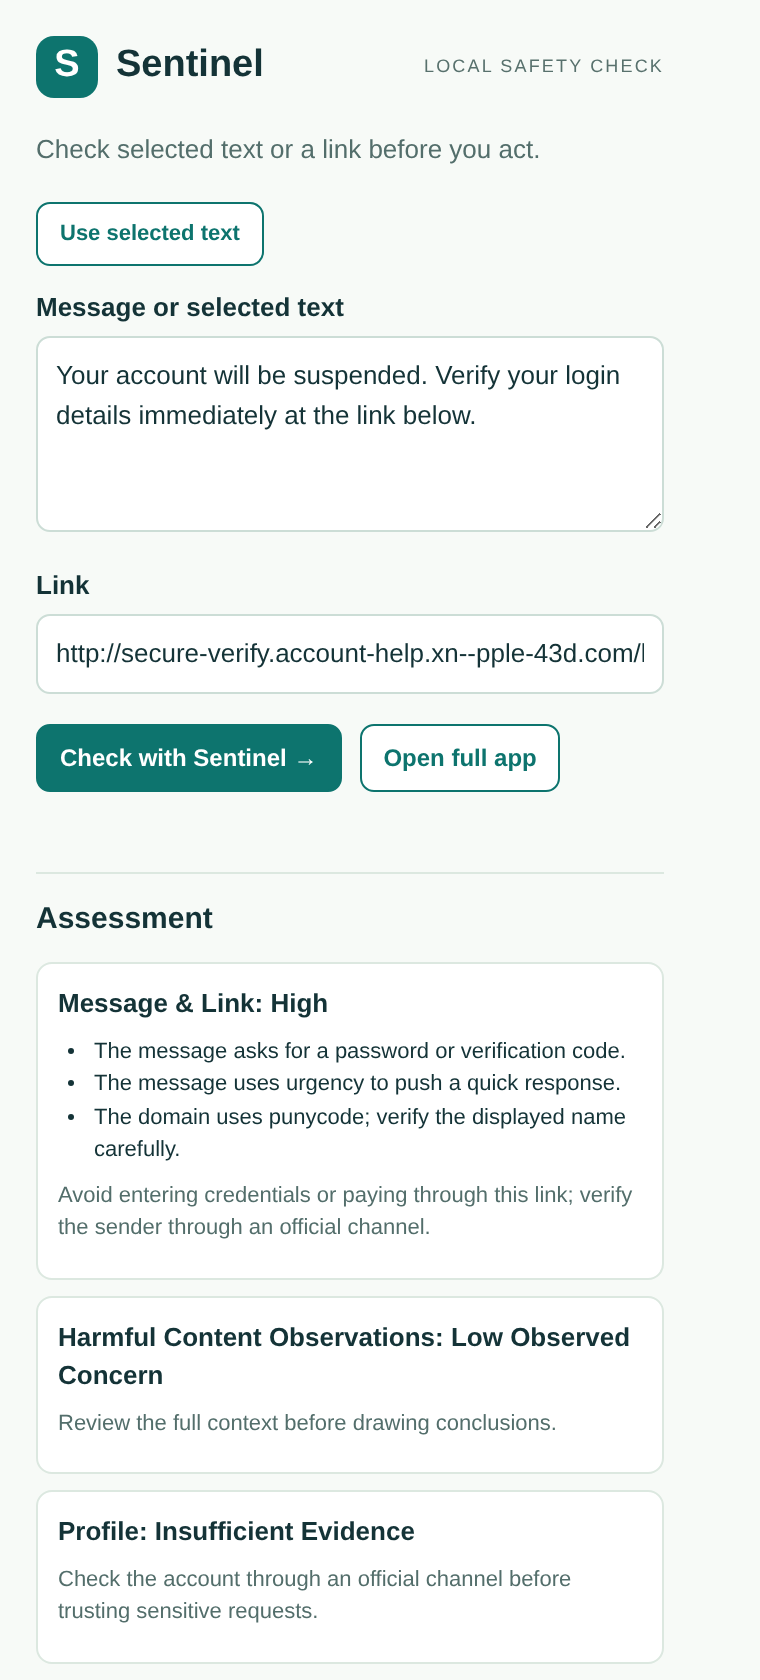
\includegraphics[width=\linewidth]{shots/13_popup_crop.png}\\[1pt]{\small (b) Extension popup}
\end{minipage}
\caption{User interface of Sentinel}
\label{fig:ui-form}
\end{figure}
\begin{figure}[H]
\centering
\begin{minipage}[t]{0.36\linewidth}\centering
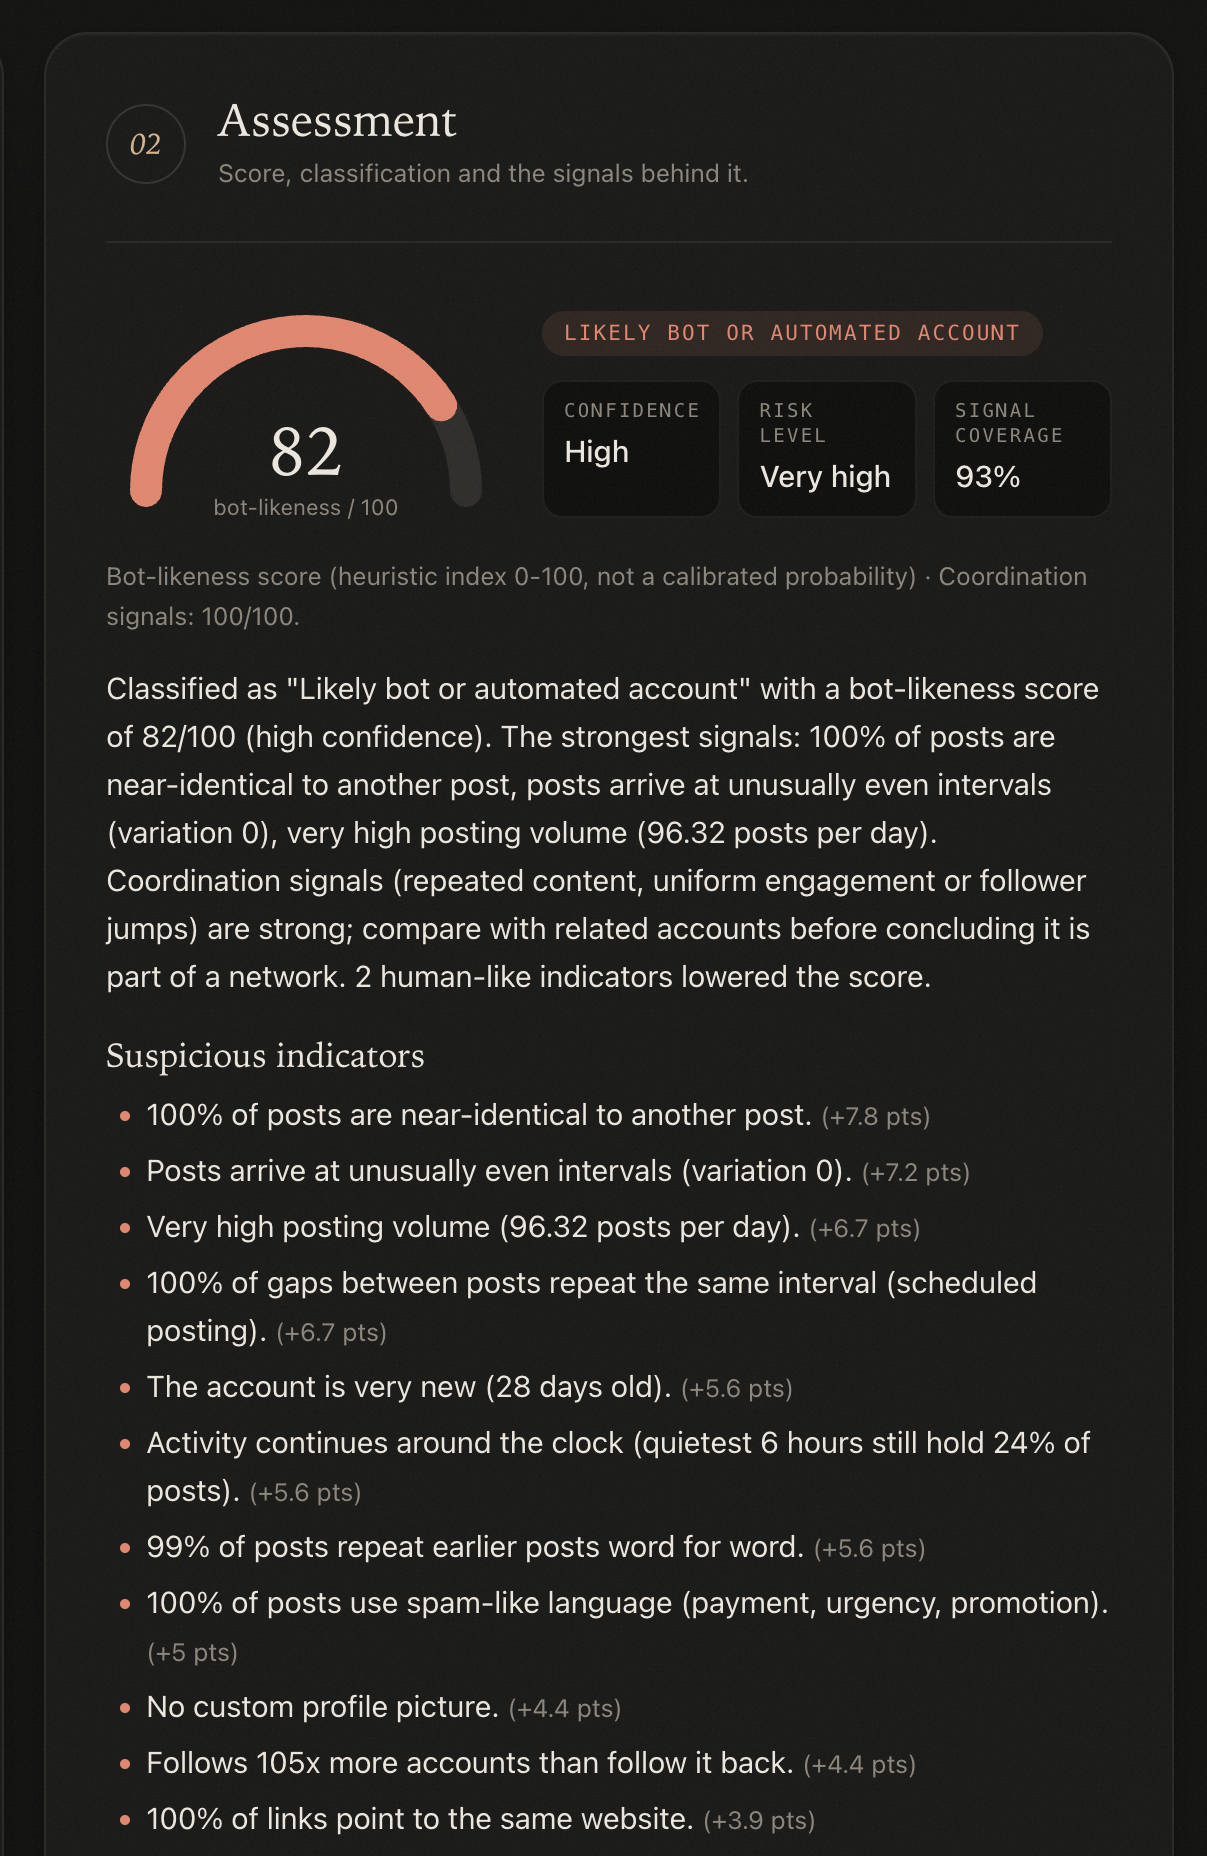
\includegraphics[width=\linewidth]{shots2/bot_report_panel.png}\\[1pt]{\small (a) Bot report for an automated account}
\end{minipage}\hfill
\begin{minipage}[t]{0.6\linewidth}\centering
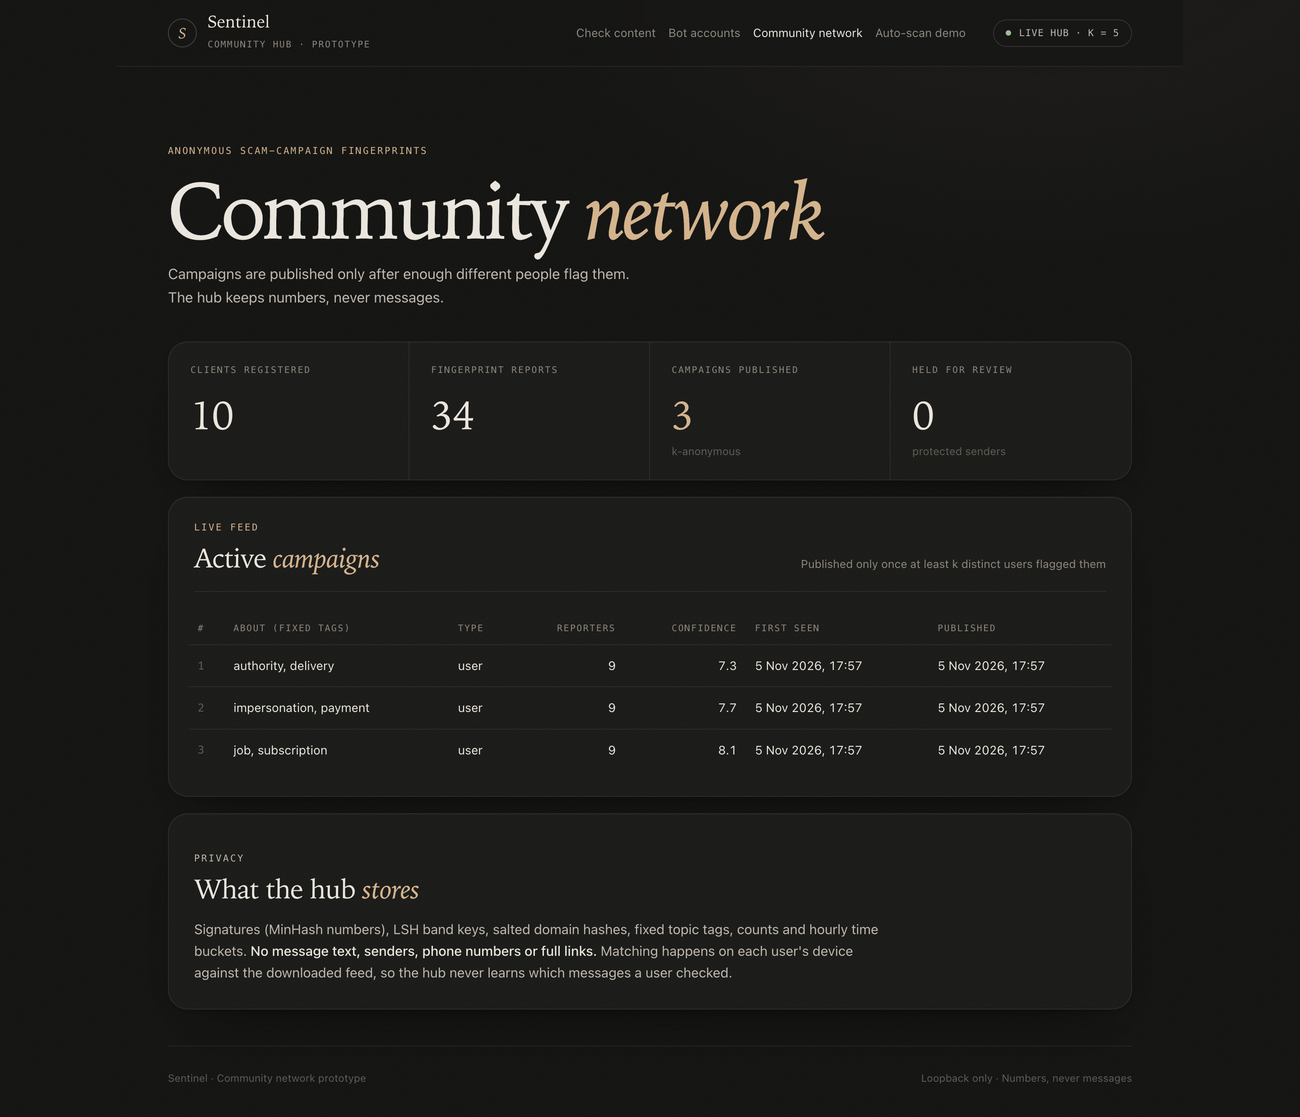
\includegraphics[width=\linewidth]{shots2/network.png}\\[1pt]{\small (b) Community network page}
\end{minipage}
\caption{Bot-detection and community-network pages}
\label{fig:ui-more}
\end{figure}

\titleformat{\chapter}[display]{\bfseries\centering}{\huge Chapter \thechapter}{1em}{\Huge #1}
\newgeometry{top=3cm, bottom=2.2cm, left=3cm, right=2cm, headsep=1.2cm, footskip=1cm, headheight=0.3cm, textheight=24.5cm, textwidth=16cm}
\onehalfspacing
\pagestyle{fancy}
\fancyhf{}
\renewcommand{\headrulewidth}{0pt}
\lhead{Chapter 4}
\rhead{Implementation Plan and Experimental Setup}
\cfoot{\thepage}
\chapter{Implementation Plan and Experimental Setup}

\section{Implementation Plan}
\noindent The project follows a twelve-month plan with a working milestone at each step (Table~\ref{tab:plan}). Work is divided into four areas: URL, message and fusion models; harmful content; profile features, data and versioning; and application, integration and deployment. Each milestone has a written plan and a delivery record in the repository \cite{repo}.

\begin{table}[H]
\centering
\small
\renewcommand{\arraystretch}{1.15}
\caption{Implementation plan and status}
\label{tab:plan}
\begin{tabular}{|>{\raggedright\arraybackslash}p{2.8cm}|>{\raggedright\arraybackslash}p{8.6cm}|>{\raggedright\arraybackslash}p{2.9cm}|}
\hline
\textbf{Phase} & \textbf{Work} & \textbf{Status} \\ \hline
Base application & Local server, web app, extension, fraud rules, saved cases & Done (Sem VII) \\ \hline
URL studies v1--v3 & Three URL models on PhiUSIIL, PhreshPhish and Mendeley data & Done; kept in research \\ \hline
Auto-scan & Opt-in page scanning, markers, badge; text in images (OCR) & Done; live \\ \hline
Scam-text model & DistilBERT + TF-IDF model, versions 1 and 2 & Done; v2 live \\ \hline
Harm rules & 19 rules for English and Hinglish & Done; live \\ \hline
Community network & Fingerprints, hub, matching, 10,000-user simulation & Done; prototype \\ \hline
Bot detection & APIs and uploads, 25-signal score, two trained models & Done; one model live \\ \hline
Research studies & Message+link study and context-aware abuse study & Software done; waiting for data \\ \hline
Semester VIII & Test on real Indian SMS; newer bot data; secure online hub; usability study with 15--20 people; final report & Planned \\ \hline
\end{tabular}
\end{table}

\section{Experimental Setup}
\subsection{Input Data and Datasets}
\noindent The application receives JSON requests from the web app or extension. The research pipeline uses public datasets, each pinned by version and checksum (Table~\ref{tab:datasets}). Raw data is kept on the team's computers and is not shared.

\begin{table}[H]
\centering
\small
\renewcommand{\arraystretch}{1.15}
\caption{Datasets used}
\label{tab:datasets}
\begin{tabular}{|>{\raggedright\arraybackslash}p{4.3cm}|>{\raggedright\arraybackslash}p{5.4cm}|>{\raggedright\arraybackslash}p{4.6cm}|}
\hline
\textbf{Dataset} & \textbf{Size} & \textbf{Used for} \\ \hline
PhiUSIIL \cite{phiusiil} & 235,795 URLs & URL study 1 \\ \hline
PhreshPhish \cite{phreshphish}, Mendeley web pages \cite{mendeley} & 666,315 and 11,430 URLs & URL studies 2 and 3 \\ \hline
SMS Phishing Dataset \cite{smsdata} & 5,971 SMS (5,790 after cleaning) & Scam-text model \\ \hline
UCI SMS Spam \cite{ucisms} & 4,908 overlapping SMS & Label cross-check only \\ \hline
Indian Scam \& Ham SMS \cite{india14} & 2,000 English/Hinglish rows (synthetic) & Scam-text model v2 \\ \hline
Bot Repository \cite{botrepo} & 13 datasets, 111,168 Twitter accounts & Profile bot model \\ \hline
cresci-2015/2017 \cite{cresci2015,cresci2017} & 10,422 accounts with post history & Activity bot model \\ \hline
CAD \cite{cad}, SpamAssassin \cite{champa} & 26,550 Reddit posts; 1,912 emails & Research studies \\ \hline
Challenge set (our own) & 44 messages written before training & Independent test \\ \hline
\end{tabular}
\end{table}

\noindent\textbf{Sample input.} A request to check content looks like this:
\begin{lstlisting}[style=json]
{ "message": "You are shortlisted for the campus internship. Pay the registration fee immediately and share the OTP to confirm your seat.",
  "url": "http://192.168.10.5/secure-login/verify" }
\end{lstlisting}

\subsection{Test Cases}
\noindent Table~\ref{tab:tests} lists the main test cases, run through the web app, the extension or the API on 30 October and 6 November 2026.

\begin{footnotesize}
\renewcommand{\arraystretch}{1.12}
\begin{longtable}{|l|>{\raggedright\arraybackslash}p{5.0cm}|>{\raggedright\arraybackslash}p{3.6cm}|>{\raggedright\arraybackslash}p{4.4cm}|}
\caption{Functional test cases}\label{tab:tests}\\
\hline
\textbf{ID} & \textbf{Input} & \textbf{Expected} & \textbf{Observed} \\ \hline
\endfirsthead
\hline
\textbf{ID} & \textbf{Input} & \textbf{Expected} & \textbf{Observed} \\ \hline
\endhead
TC-01 & Fake internship asking for fee and OTP, IP-address link & Fraud High & High, 4 pieces of evidence (Pass) \\ \hline
TC-02 & ``I will kill you tomorrow after school'' & Harm High (threat) & High, threat of violence (Pass) \\ \hline
TC-03 & Someone wrote ``you are stupid'' (quoted) & Harm Review & Review, asks for human review (Pass) \\ \hline
TC-04 & ``tu pagal hai kya, chal nikal bewakoof'' (Hinglish) & Harm Review & Review, Hinglish insult (Pass) \\ \hline
TC-05 & ``This movie killed it''; ``I would never hurt you'' & Not flagged & Low concern for both (Pass) \\ \hline
TC-06 & ``i want to end my life tonight'' & Harm High with helpline & High; Tele-MANAS 14416 shown (Pass) \\ \hline
TC-07 & ``k.y.s loser'' (disguised) & Harm High & High, self-harm encouragement (Pass) \\ \hline
TC-08 & Parcel-fee scam with IP-address link & Fraud High; model flags & High; model 98.4\% smishing (Pass) \\ \hline
TC-09 & Genuine OTP message; genuine UPI debit alert & Model does not flag & OTP: not flagged (Pass); debit alert: flagged 72\% (Fail) \\ \hline
TC-10 & Auto-scan: taunt, insult, lunch message, scam & high, review, none, high & Exactly as expected (Pass) \\ \hline
TC-11 & Bot check of \texttt{x.com@evil.com} & Rejected & 400 error, no network access (Pass) \\ \hline
TC-12 & Uploaded bot-like and human-like accounts & Bot / human & 82/100 bot; 4/100 human (Pass) \\ \hline
TC-13 & YouTube check with no API key & Clear error & ``Set YOUTUBE\_API\_KEY'' (Pass) \\ \hline
TC-14 & Empty request; body over 200 KB; wrong content type & Error 400 & 400 with a clear message (Pass) \\ \hline
TC-15 & Request from another website & Error 403 & 403 (Pass) \\ \hline
TC-16 & Save with a forged receipt & Rejected & ``Recheck this content'' (Pass) \\ \hline
TC-17 & Save, give feedback, delete twice & Saved; then 404 & Saved; second delete 404 (Pass) \\ \hline
\end{longtable}
\end{footnotesize}

\noindent\textbf{Automated tests.} On 6 November 2026, 112 Python application tests and 76 JavaScript tests passed. The full research suite ran 569 tests: 519 passed, 7 were skipped and 43 failed; all 43 need Windows-only features and pass in the project's Windows setup.

\subsection{Performance Evaluation Parameters}
\noindent With $TP$, $FP$, $TN$ and $FN$ the counts of true and false positives and negatives:
\begin{align}
\text{Precision} &= \frac{TP}{TP+FP}, &
\text{Recall} &= \frac{TP}{TP+FN}, &
F_1 &= \frac{2TP}{2TP+FP+FN}, &
\text{FPR} &= \frac{FP}{FP+TN}.
\end{align}
\textbf{Precision} is how many warnings were right; \textbf{recall} is how many scams were caught; \textbf{FPR} (false-positive rate) is how many genuine items were wrongly flagged. \textbf{Macro-F1} averages $F_1$ over the classes. \textbf{ROC AUC} is the chance that a random bot scores higher than a random human (0.5 = guessing, 1 = perfect). \textbf{Calibration error (ECE)} measures how far the stated probabilities are from reality. For bots, the release test uses the \emph{worst} score over datasets the model never saw.

\section{Partial Code}
\noindent\textbf{Fraud level} (\texttt{sentinel/analysis.py}):
\lstinputlisting[style=py, firstline=107, lastline=122, firstnumber=107]{Code/analysis.py}

\titleformat{\chapter}[display]{\bfseries\centering}{\huge Chapter \thechapter}{1em}{\Huge #1}
\newgeometry{top=3cm, bottom=2.2cm, left=3cm, right=2cm, headsep=1.2cm, footskip=1cm, headheight=0.3cm, textheight=24.5cm, textwidth=16cm}
\onehalfspacing
\pagestyle{fancy}
\fancyhf{}
\renewcommand{\headrulewidth}{0pt}
\lhead{Chapter 5}
\rhead{Results and Discussions}
\cfoot{\thepage}
\chapter{Results and Discussions}

\section{Application Results}
\noindent 16 of the 17 test cases in Table~\ref{tab:tests} passed. The one failure (TC-09) is a known weakness of the text model, explained in Section~\ref{sec:textres}. Figure~\ref{fig:res-harm} shows the harm results for a direct threat and for a quoted insult.

\begin{figure}[H]
\centering
\begin{minipage}[t]{0.62\linewidth}\centering
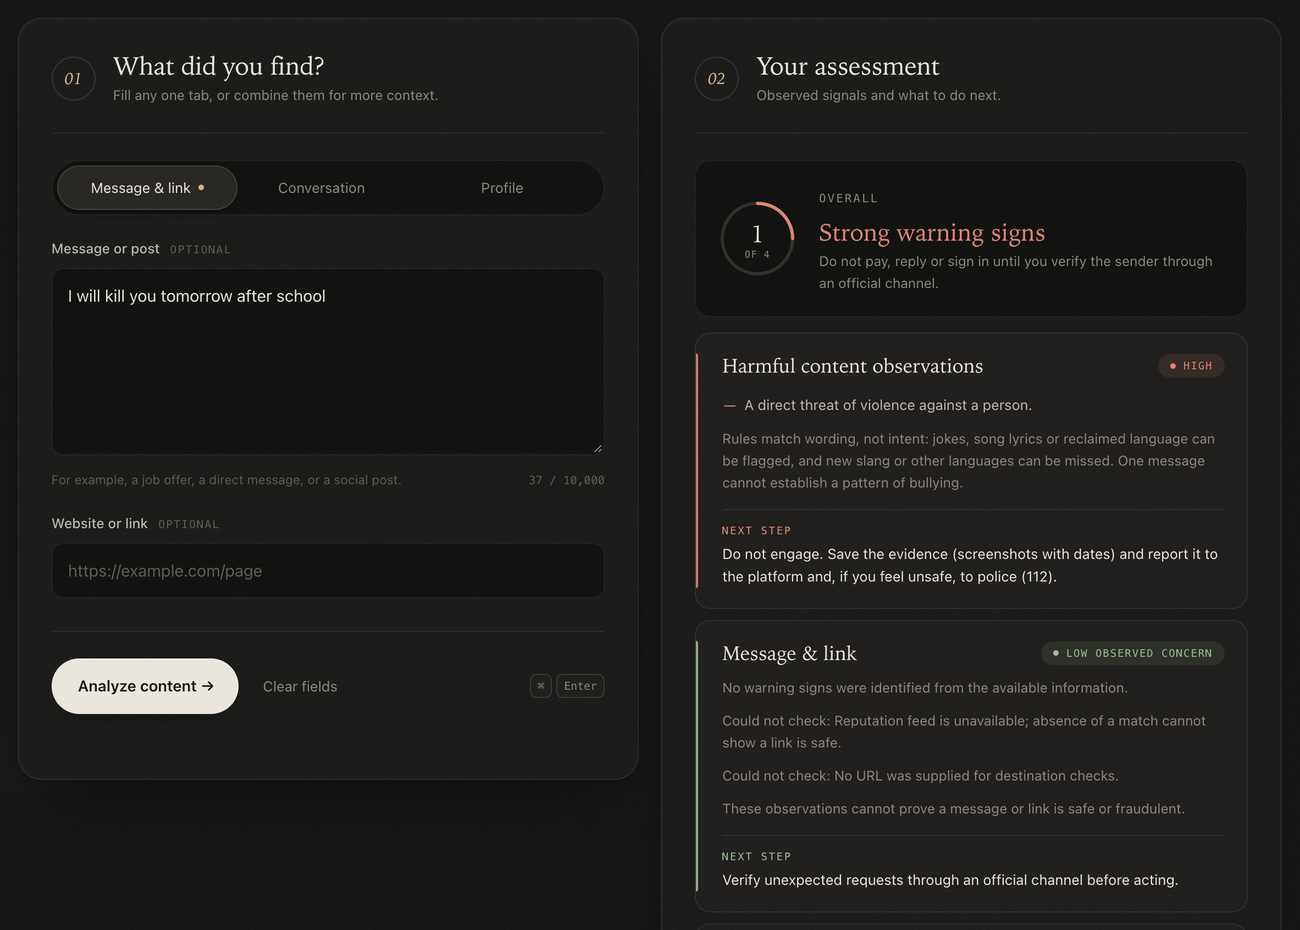
\includegraphics[width=\linewidth]{shots2/check_threat.png}\\[1pt]{\small (a) Direct threat: the harm card moves to the top}
\end{minipage}\hfill
\begin{minipage}[t]{0.30\linewidth}\centering
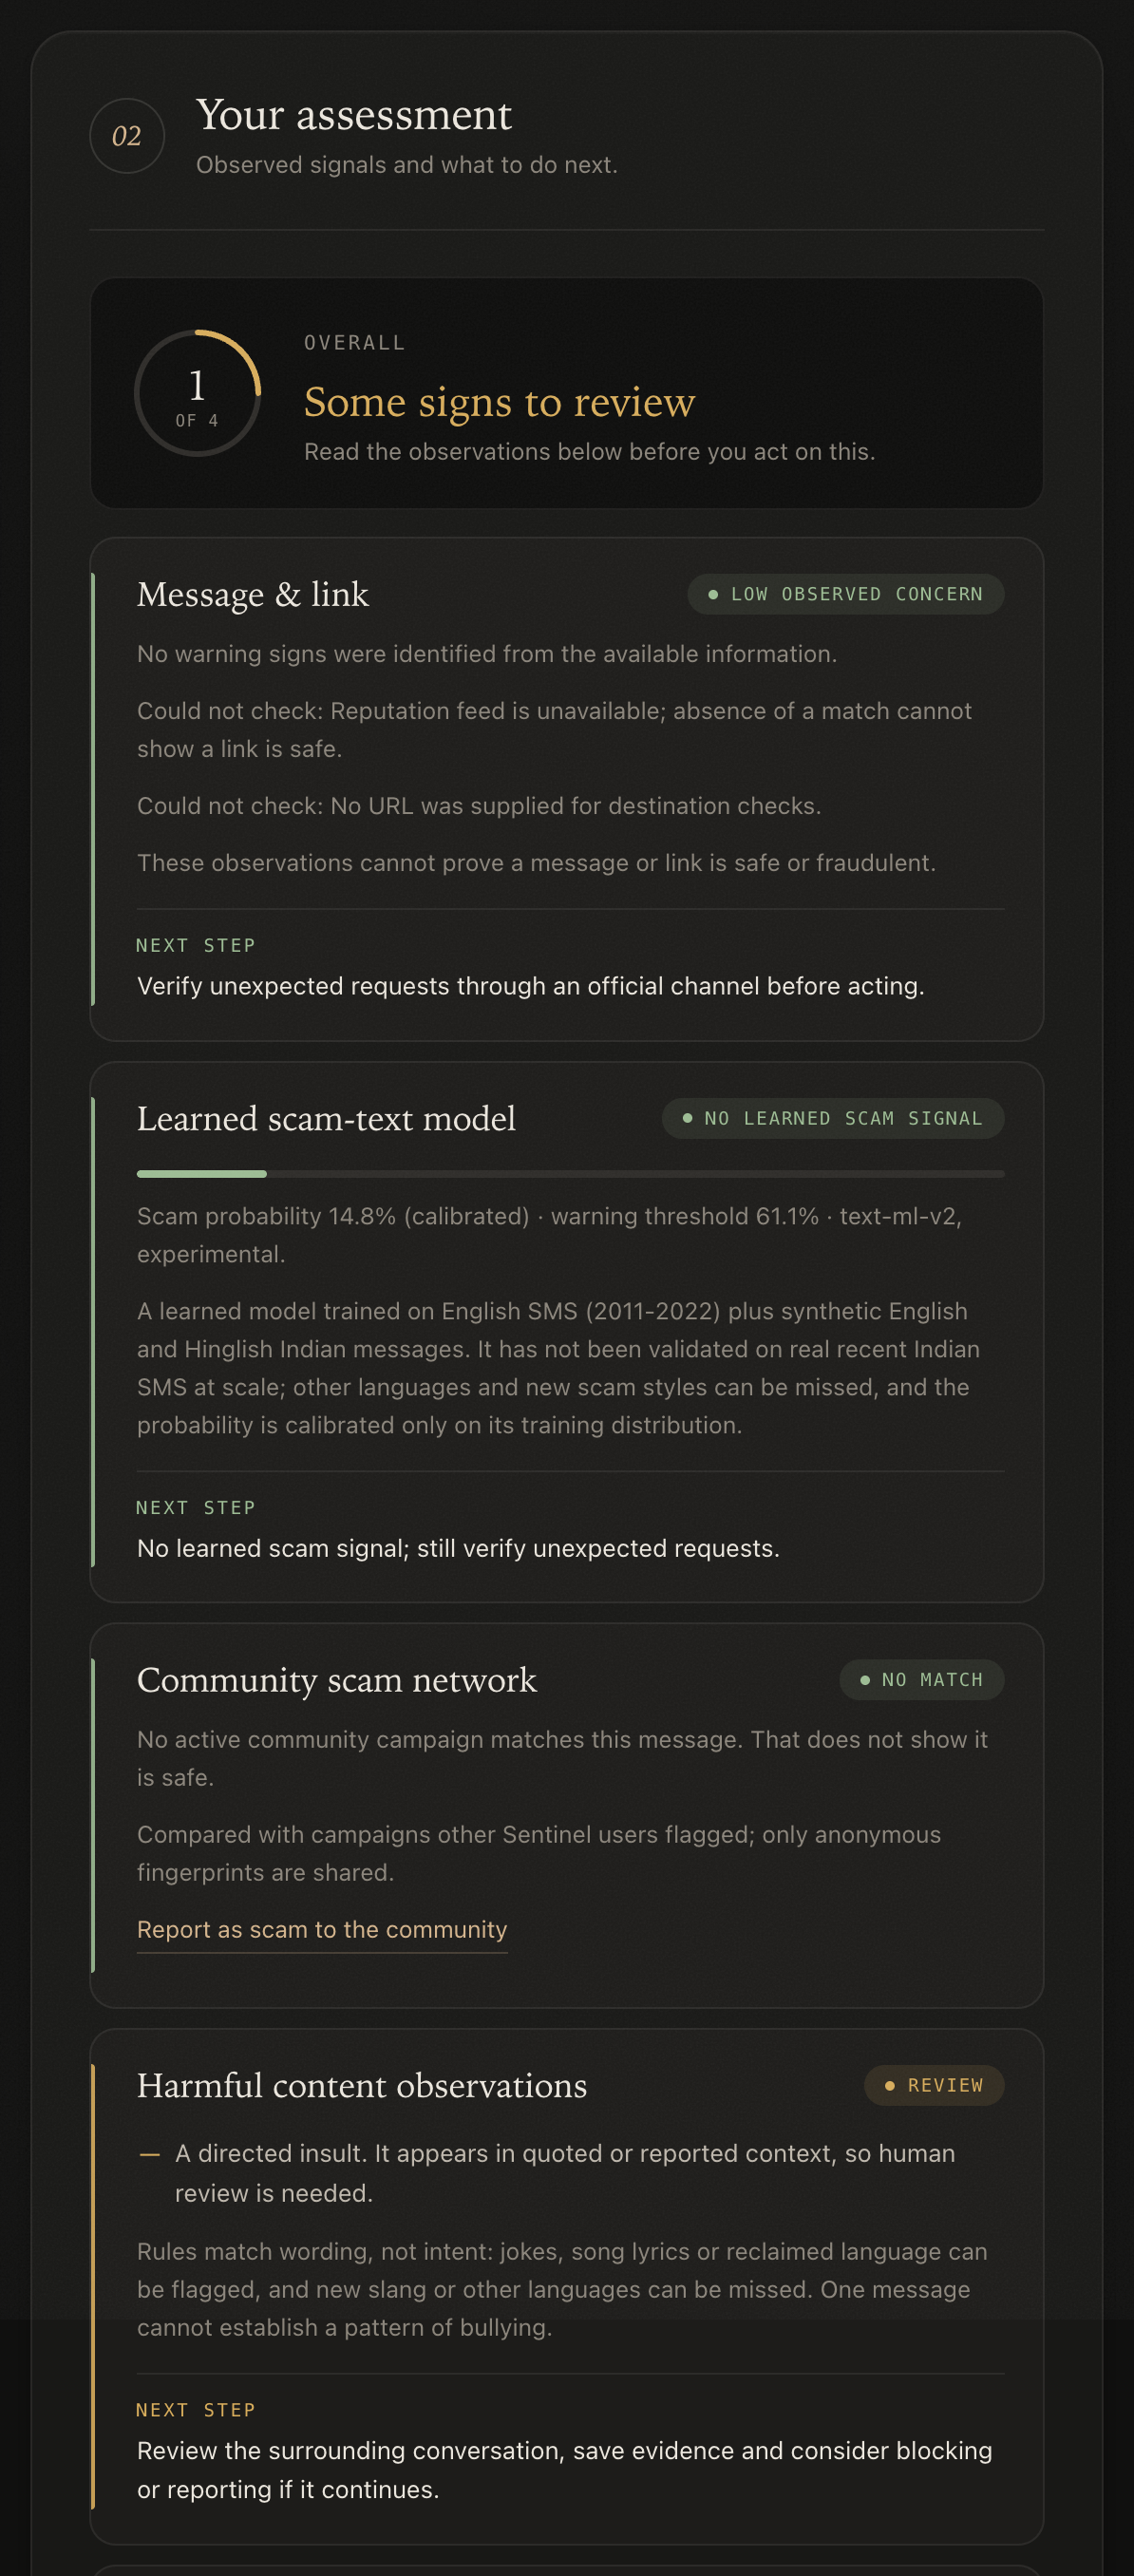
\includegraphics[width=\linewidth]{shots2/check_quoted.png}\\[1pt]{\small (b) Quoted insult: sent for human review}
\end{minipage}
\caption{Harmful-language results for a direct threat and a quoted insult}
\label{fig:res-harm}
\end{figure}

\noindent\textbf{Observations.}
\begin{itemize}
\item The fake internship (TC-01) was rated High by the rules, but the text model gave it only 56\%, below its 61.1\% threshold. This is why the model is shown \emph{next to} the rules and never replaces them.
\item Threats are rated High with clear advice; quoted insults go to human review instead of blaming the writer.
\item Rule checks finish in about a millisecond, so results feel instant.
\end{itemize}

\section{Scam-Text Model}\label{sec:textres}
\noindent Version 1 of the model scored well on its own test set, but our community-network simulation showed that it wrongly flagged 91--99\% of genuine Indian bank and OTP messages, because its training data had almost no genuine business messages. Version 2 added 2,000 Indian-style messages (synthetic) and averages two models. Table~\ref{tab:text} compares them.

\begin{table}[H]
\centering
\small
\renewcommand{\arraystretch}{1.15}
\caption{Scam-text model results}
\label{tab:text}
\begin{tabular}{|l|c|c|c|c|}
\hline
\textbf{Model} & \textbf{Macro-F1} & \textbf{Genuine flagged} & \multicolumn{2}{c|}{\textbf{Challenge set (44 msgs)}} \\
 & \textbf{(870 SMS)} & \textbf{(870 SMS)} & \textbf{Genuine flagged} & \textbf{Scams caught} \\ \hline
text-ml-v1 & 0.896 & 0 / 725 & 17 / 24 & 14 / 20 \\ \hline
\textbf{text-ml-v2} & \textbf{0.897} & \textbf{0 / 725} & \textbf{2 / 24} & \textbf{14 / 20} \\ \hline
\end{tabular}
\end{table}

\noindent Version 2 kept the same accuracy on the original test and cut false alarms on genuine Indian messages from 17 of 24 to 2 of 24. It runs in about 2 ms per message. \textbf{Limits:} the challenge set is small; the new data is synthetic; and the model still misses chat-style scams (``new number, send money'') and flags some genuine bank alerts.

\section{Harmful-Language Rules}
\noindent The old rule caught only 2 of 11 harmful test sentences. The new engine is tested on 12 high-risk sentences, 8 insults and 13 harmless sentences (idioms, negations and everyday Hinglish), and all are handled correctly. Because rules match words, not intent, new slang can still be missed.

\section{Auto-Scan Extension}
\noindent In TC-10 every page item got the expected severity. On the demo chat page the extension marked the job-fee, OTP and bank-login scams and the anonymous insult, and new messages were scanned as they appeared. A page scan takes about 190 ms. With image reading on, it also flagged the three scam images on the demo page, ignored the harmless one and read the link inside a QR code.

\section{Community Scam Network}
\noindent We simulated 10,000 users for 72 hours with 30 scam campaigns that are reworded every 6 hours and 12 genuine bulk messages.

\begin{table}[H]
\centering
\small
\renewcommand{\arraystretch}{1.15}
\caption{Share of scam messages that were warned}
\label{tab:net1}
\begin{tabular}{|l|c|c|}
\hline
\textbf{Detector on each device} & \textbf{Model alone} & \textbf{Model + network} \\ \hline
Simulated detector & 78.2\% & 99.7\% \\ \hline
text-ml-v2 (real model) & 86.0\% & 93.1\% \\ \hline
\end{tabular}
\end{table}

\begin{figure}[H]
\centering
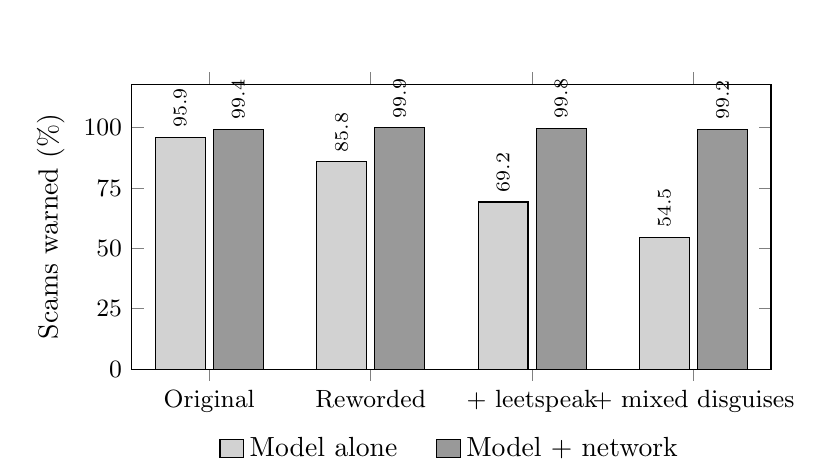
\begin{tikzpicture}
\begin{axis}[ybar=3pt, bar width=18pt, width=0.8\linewidth, height=5.2cm, ymin=0, ymax=118, ytick={0,25,50,75,100}, ylabel={Scams warned (\%)},
  symbolic x coords={Original,Reworded,+ leetspeak,+ mixed disguises}, xtick=data, enlarge x limits=0.16,
  legend style={at={(0.5,-0.2)}, anchor=north, legend columns=2, draw=none, /tikz/every even column/.append style={column sep=12pt}}, legend image code/.code={\draw[#1] (0cm,-0.1cm) rectangle (0.3cm,0.12cm);},
  nodes near coords, nodes near coords style={font=\scriptsize, rotate=90, anchor=west}, point meta=y,
  every axis plot/.append style={draw=black}, tick label style={font=\small}]
\addplot[fill=gray!35] coordinates {(Original,95.9) (Reworded,85.8) (+ leetspeak,69.2) (+ mixed disguises,54.5)};
\addplot[fill=gray!80] coordinates {(Original,99.4) (Reworded,99.9) (+ leetspeak,99.8) (+ mixed disguises,99.2)};
\legend{Model alone, Model + network}
\end{axis}
\end{tikzpicture}
\caption{Protection as scams get more disguised (simulated detector)}
\label{fig:netmut}
\end{figure}

\noindent As scams get more disguised, each user's own detector gets worse, but the network keeps protection near 99\% (Figure~\ref{fig:netmut}). The biggest risk we found was not attackers but honest mistakes at scale: a genuine message sent to thousands of people can collect several false reports. Without defences, 54.4\% of genuine bulk messages got a wrong warning; with the verified-sender list and user disputes, only 2.4\%. No message text was ever found in the hub's database.

\section{Bot-Account Detection}
\noindent Both trained models had to reach an AUC of at least 0.80 on \emph{every} dataset they had never seen (Table~\ref{tab:bot}).

\begin{table}[H]
\centering
\small
\renewcommand{\arraystretch}{1.15}
\caption{Bot models: results on unseen data}
\label{tab:bot}
\begin{tabular}{|>{\raggedright\arraybackslash}p{3.8cm}|>{\raggedright\arraybackslash}p{3.4cm}|c|c|c|}
\hline
\textbf{Model} & \textbf{Data} & \textbf{AUC, mixed data} & \textbf{Worst unseen AUC} & \textbf{Decision} \\ \hline
Profile model (bot-ml-v1) & 111,168 accounts, profile details & 0.967 & 0.600 & Failed: hidden \\ \hline
Activity model (bot-ml-activity-v1) & 10,422 accounts, posting behaviour & 0.997 & 0.849 & Passed: live \\ \hline
\end{tabular}
\end{table}

\noindent The profile model looked excellent on mixed data (0.967) but dropped to 0.600 on a dataset it had not seen, so it is not used. The activity model passed: it even caught human-like spambots it had never seen (AUC 0.981), where our hand-made score was worse than guessing (0.157). Its limit is that it learned from Twitter accounts of 2009--2017.

\section{URL Studies (Research Only)}
\noindent The first URL model reached 97.07\% F1 on PhiUSIIL, but all genuine URLs in that dataset were home pages, so the model learned the format rather than the fraud. The third model reached 92.71\% F1 on the larger PhreshPhish data, but still wrongly flagged 22.39\% of genuine links on a second test set (Figure~\ref{fig:v3}). Both are kept out of the application.
\begin{figure}[H]
\centering
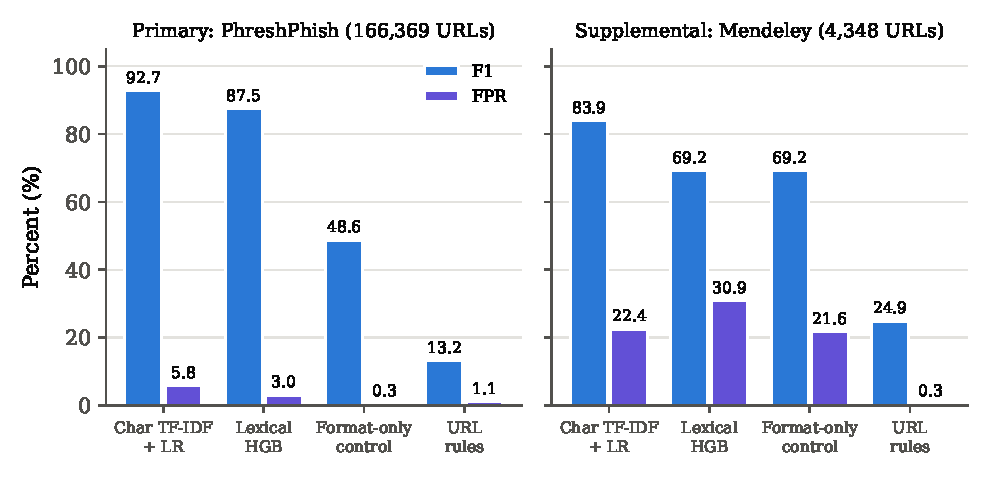
\includegraphics[width=0.78\linewidth]{charts/c5_v3_tracks.pdf}
\caption{URL model v3: F1 and false-positive rate on the two test sets}
\label{fig:v3}
\end{figure}
\noindent The message+link study has no real data yet, and the context-aware abuse study on CAD stopped because the data did not meet its minimum size rules, so no model was trained.

\section{Comparison with Existing Systems}
\begin{table}[H]
\centering
\small
\renewcommand{\arraystretch}{1.15}
\caption{Reported results of existing work and Sentinel (different tasks, shown for context)}
\label{tab:compare}
\begin{tabular}{|>{\raggedright\arraybackslash}p{3.6cm}|>{\raggedright\arraybackslash}p{4.2cm}|>{\raggedright\arraybackslash}p{5.6cm}|}
\hline
\textbf{System} & \textbf{Task} & \textbf{Result} \\ \hline
Aditya and Mohanty \cite{lit2} & Fake profiles (platform data) & 93.5\% accuracy \\ \hline
Atif et al. \cite{lit4} & Roman Urdu bullying & 97\% F1 \\ \hline
Sentinel text-ml-v2 & SMS scams & Macro-F1 0.897; 0 of 725 genuine flagged \\ \hline
Sentinel activity bot model & Twitter bots & Worst unseen AUC 0.849 \\ \hline
Sentinel URL v1 / v3 & Phishing URLs & 97.07\% / 92.71\% F1 (not live) \\ \hline
\end{tabular}
\end{table}
\noindent The tasks differ, so these numbers cannot be compared directly. Unlike the cited work, Sentinel tests on data its models have never seen. As Table~\ref{tab:features} shows, it is also the only system that combines all these checks, runs locally and explains its results.

\section{Discussion}
\noindent The application works as planned. Two learned models passed their tests and are live; two others failed and were kept out, which shows the testing process doing its job. The main lesson is that a high score is not enough: the URL model's 97\% and the profile bot model's 0.967 both hid weaknesses that only fair testing revealed.

\titleformat{\chapter}[display]{\bfseries\centering}{\huge Chapter \thechapter}{1em}{\Huge #1}
\newgeometry{top=3cm, bottom=2.2cm, left=3cm, right=2cm, headsep=1.2cm, footskip=1cm, headheight=0.3cm, textheight=24.5cm, textwidth=16cm}
\onehalfspacing
\pagestyle{fancy}
\fancyhf{}
\renewcommand{\headrulewidth}{0pt}
\lhead{Chapter 6}
\rhead{Conclusion}
\cfoot{\thepage}
\chapter{Conclusion}

\section{Summary of Work Completed in Major Project Part 1 (Semester VII)}
\noindent Sentinel helps an ordinary social-media user judge a suspicious message, link or account before acting on it, without sending their data away. In Semester VII the team built:
\begin{enumerate}
\item \textbf{A working local application:} a web app and a Chrome extension that give separate, explained results for fraud, harmful language and accounts.
\item \textbf{Harm detection} for English and Hinglish that handles disguised words, quotes and idioms, and gives helpline numbers for self-harm.
\item \textbf{A learned scam-text model} (v2) that keeps its accuracy and cuts false alarms on genuine Indian messages from 17 of 24 to 2 of 24.
\item \textbf{Auto-scan,} which marks risky text and images on sites the user chooses.
\item \textbf{A community network} that raised protection from 78.2\% to 99.7\% in a 10,000-user simulation without sharing message text.
\item \textbf{Bot detection} from official APIs or user data, with one model released (worst unseen AUC 0.849) and one held back (0.600).
\item \textbf{A fair testing process} with three URL studies and model cards, which kept weak models out of the application.
\end{enumerate}

\section{Limitations}
\begin{itemize}
\item Rules match words, not intent, and can miss new slang.
\item The scam model's Indian data is synthetic, and it still misses chat-style scams.
\item The bot model learned from older Twitter data.
\item The community hub runs on one computer and has no login system yet.
\end{itemize}

\section{Future Work (Semester VIII)}
\begin{enumerate}
\item Test the scam model on real, consented Indian SMS and add modern scam types.
\item Add newer bot data (TwiBot-22) and support more platforms.
\item Move the community hub online with secure logins.
\item Run a usability study with 15--20 volunteers before the final release.
\end{enumerate}

\titleformat{\chapter}[display]{\bfseries\centering}{\huge Chapter \thechapter}{1em}{\Huge #1}
\pagestyle{fancy}
\fancyhf{}
\renewcommand{\headrulewidth}{0pt}
\lhead{Chapter 7}
\rhead{References}
\cfoot{\thepage}
\chapter{References}
\onehalfspacing
\begin{thebibliography}{99}

\bibitem{lit1} R. Bhambulkar, S. Choudhary, and A. Pimpalkar, ``Detecting fake profiles on social networks: A systematic investigation,'' in \textit{Proc. 2023 IEEE Int. Students' Conf. Electrical, Electronics and Computer Science (SCEECS)}, 2023, pp. 1--6, doi: 10.1109/SCEECS57921.2023.10063046.

\bibitem{lit2} B. L. V. S. Aditya and S. N. Mohanty, ``Heterogenous social media analysis for efficient deep learning fake-profile identification,'' \textit{IEEE Access}, vol. 11, pp. 99339--99351, 2023, doi: 10.1109/ACCESS.2023.3313169.

\bibitem{lit3} A. K. M. R. R. Habib, E. E. Akpan, B. Ghosh, and I. K. Dutta, ``Techniques to detect fake profiles on social media using the new age algorithms -- A survey,'' in \textit{Proc. 2024 IEEE 14th Annu. Computing and Communication Workshop and Conf. (CCWC)}, 2024, pp. 329--335, doi: 10.1109/CCWC60891.2024.10427620.

\bibitem{lit4} A. Atif \textit{et al.}, ``Cyberbullying detection and abuser profile identification on social media for Roman Urdu,'' \textit{IEEE Access}, vol. 12, pp. 123339--123351, 2024, doi: 10.1109/ACCESS.2024.3445288.

\bibitem{lit5} Y. M. Ibrahim, R. Essameldin, and S. M. Saad, ``Social media forensics: An adaptive cyberbullying-related hate speech detection approach based on neural networks with uncertainty,'' \textit{IEEE Access}, vol. 12, pp. 59474--59484, 2024, doi: 10.1109/ACCESS.2024.3393295.

\bibitem{phiusiil} A. Prasad and S. Chandra, ``PhiUSIIL: A diverse security profile empowered phishing URL detection framework based on similarity index and incremental learning,'' \textit{Computers \& Security}, 2024, Art. no. 103545, doi: 10.1016/j.cose.2023.103545.

\bibitem{cad} B. Vidgen, D. Nguyen, H. Margetts, P. Rossini, and R. Tromble, ``Introducing CAD: the Contextual Abuse Dataset,'' in \textit{Proc. 2021 Conf. North American Chapter of the Association for Computational Linguistics: Human Language Technologies (NAACL-HLT)}, 2021, pp. 2289--2303, doi: 10.18653/v1/2021.naacl-main.182.

\bibitem{phreshphish} T. Dalton \textit{et al.}, ``PhreshPhish: A real-world, high-quality, large-scale phishing website dataset and benchmark,'' arXiv:2507.10854, 2025.

\bibitem{mendeley} A. Hannousse and S. Yahiouche, ``Web page phishing detection,'' Mendeley Data, V3, 2021, doi: 10.17632/c2gw7fy2j4.3.

\bibitem{champa} A. I. Champa, M. F. Rabbi, and M. F. Zibran, ``Curated datasets and feature analysis for phishing email detection with machine learning,'' in \textit{Proc. 3rd IEEE Int. Conf. Computing and Machine Intelligence (ICMI)}, 2024, pp. 1--7.

\bibitem{distilbert} V. Sanh, L. Debut, J. Chaumond, and T. Wolf, ``DistilBERT, a distilled version of BERT: Smaller, faster, cheaper and lighter,'' arXiv:1910.01108, 2019.

\bibitem{sklearn} F. Pedregosa \textit{et al.}, ``Scikit-learn: Machine learning in Python,'' \textit{J. Mach. Learn. Res.}, vol. 12, pp. 2825--2830, 2011.

\bibitem{guo} C. Guo, G. Pleiss, Y. Sun, and K. Q. Weinberger, ``On calibration of modern neural networks,'' in \textit{Proc. 34th Int. Conf. Machine Learning (ICML)}, 2017, pp. 1321--1330.

\bibitem{homograph} E. Gabrilovich and A. Gontmakher, ``The homograph attack,'' \textit{Commun. ACM}, vol. 45, no. 2, p. 128, 2002.

\bibitem{hmac} H. Krawczyk, M. Bellare, and R. Canetti, ``HMAC: Keyed-hashing for message authentication,'' RFC 2104, IETF, 1997.

\bibitem{phishtank} Cisco Talos Intelligence Group, ``PhishTank developer information.'' [Online]. Available: \url{https://phishtank.org/developer_info.php}

\bibitem{safebrowsing} Google, ``Safe Browsing APIs.'' [Online]. Available: \url{https://developers.google.com/safe-browsing}

\bibitem{mv3} Google, ``Extensions / Manifest V3,'' Chrome for Developers. [Online]. Available: \url{https://developer.chrome.com/docs/extensions/develop/migrate/what-is-mv3}

\bibitem{repo} Sentinel project team, ``Sentinel: Source code, model cards and delivery records,'' project repository. [Online]. Available: \url{https://github.com/jasondsouza27/sentinel}

\bibitem{cresci2015} S. Cresci, R. Di Pietro, M. Petrocchi, A. Spognardi, and M. Tesconi, ``Fame for sale: Efficient detection of fake Twitter followers,'' \textit{Decision Support Systems}, vol. 80, pp. 56--71, 2015.

\bibitem{cresci2017} S. Cresci, R. Di Pietro, M. Petrocchi, A. Spognardi, and M. Tesconi, ``The paradigm-shift of social spambots: Evidence, theories, and tools for the arms race,'' in \textit{Proc. 26th Int. Conf. World Wide Web Companion}, 2017, pp. 963--972.

\bibitem{yang2020} K.-C. Yang, O. Varol, P.-M. Hui, and F. Menczer, ``Scalable and generalizable social bot detection through data selection,'' in \textit{Proc. AAAI Conf. Artificial Intelligence}, vol. 34, no. 1, 2020, pp. 1096--1103.

\bibitem{smsdata} S. Mishra and D. Soni, ``SMS phishing dataset for machine learning and pattern recognition,'' Mendeley Data, V1, 2022, doi: 10.17632/f45bkkt8pr.1.

\bibitem{ucisms} T. Almeida and J. Hidalgo, ``SMS Spam Collection,'' UCI Machine Learning Repository, 2011, doi: 10.24432/C5CC84.

\bibitem{india14} anmolshrivastav, ``Indian multilingual scam and ham SMS (14 languages),'' Hugging Face dataset, revision 34e2c41, MIT licence. [Online]. Available: \url{https://huggingface.co/datasets/anmolshrivastav/scam_ham_india_14_languages}

\bibitem{botrepo} Observatory on Social Media, Indiana University, ``Bot Repository.'' [Online]. Available: \url{https://botometer.osome.iu.edu/bot-repository/}

\bibitem{broder} A. Z. Broder, ``On the resemblance and containment of documents,'' in \textit{Proc. Compression and Complexity of SEQUENCES 1997}, 1997, pp. 21--29.

\bibitem{mmds} J. Leskovec, A. Rajaraman, and J. D. Ullman, \textit{Mining of Massive Datasets}, 3rd ed. Cambridge, U.K.: Cambridge University Press, 2020.

\bibitem{sweeney} L. Sweeney, ``$k$-anonymity: A model for protecting privacy,'' \textit{Int. J. Uncertainty, Fuzziness and Knowledge-Based Systems}, vol. 10, no. 5, pp. 557--570, 2002.

\bibitem{zadrozny} B. Zadrozny and C. Elkan, ``Transforming classifier scores into accurate multiclass probability estimates,'' in \textit{Proc. 8th ACM SIGKDD Int. Conf. Knowledge Discovery and Data Mining}, 2002, pp. 694--699.

\bibitem{telemanas} Ministry of Health and Family Welfare, Government of India, ``Tele-MANAS: Tele Mental Health Assistance and Networking Across States (helpline 14416).'' [Online]. Available: \url{https://telemanas.mohfw.gov.in}

\end{thebibliography}

\newpage
\chapter*{Appendix-I}
\addcontentsline{toc}{chapter}{Appendix-I: API Reference}
\onehalfspacing
\pagestyle{fancy}
\fancyhf{}
\renewcommand{\headrulewidth}{0pt}
\lhead{Appendix-I}
\rhead{API Reference}
\cfoot{\thepage}
\renewcommand{\thetable}{A.\arabic{table}}\setcounter{table}{0}
\noindent The local Sentinel service listens on \texttt{http://127.0.0.1:8787}. Requests must carry the local Host header; browser requests that send an Origin are accepted only from the service's own origin or a Chrome-extension origin. JSON bodies must be between 1 and 200,000 bytes (3 MB for \texttt{/api/bot/analyze}).

\begin{table}[H]
\centering
\small
\renewcommand{\arraystretch}{1.2}
\caption{Sentinel API endpoints (the optional hub on port 8790 adds \texttt{/v1/register}, \texttt{/v1/reports}, \texttt{/v1/disputes}, \texttt{/v1/campaigns} and \texttt{/v1/stats})}
\label{tab:api}
\begin{tabular}{|l|l|>{\raggedright\arraybackslash}p{8.6cm}|}
\hline
\textbf{Method} & \textbf{Path} & \textbf{Purpose} \\ \hline
GET & \texttt{/api/health} & Service status, whether a reputation feed or research models are loaded \\ \hline
POST & \texttt{/api/analyze} & Analyse a message, URL, conversation and/or profile; returns assessments and a signed receipt \\ \hline
POST & \texttt{/api/cases} & Save a reviewed input and result with its receipt \\ \hline
GET & \texttt{/api/cases} & List saved cases, newest first \\ \hline
GET & \texttt{/api/cases/\{id\}} & Open one saved case \\ \hline
GET & \texttt{/api/cases/\{id\}/report} & Export a saved case as JSON \\ \hline
POST & \texttt{/api/cases/\{id\}/feedback} & Record \texttt{correct}, \texttt{incorrect} or \texttt{unsure} with an optional note \\ \hline
DELETE & \texttt{/api/cases/\{id\}} & Delete a saved case \\ \hline
POST & \texttt{/api/scan} & Auto-scan: up to 40 page items; returns a severity, evidence and action for each \\ \hline
POST & \texttt{/api/community/report} & Report a scam to the community hub as a fingerprint (opt-in) \\ \hline
GET & \texttt{/api/bot/platforms} & Supported platforms and whether their API keys are configured \\ \hline
POST & \texttt{/api/bot/analyze} & Analyse an account from an official API, an upload or manual entry \\ \hline
GET & \texttt{/v1/stats}, \texttt{/v1/campaigns} & Read-only forward of the hub's statistics and published campaigns (for the Community network page) \\ \hline
GET & \texttt{/}, \texttt{/bot}, \texttt{/network}, \texttt{/demo} & Web pages and their static assets \\ \hline
\end{tabular}
\end{table}

\noindent\textbf{Running the application.}
\begin{lstlisting}[style=json]
# full application: text model and bot models (uses .venv-text-ml)
./start-sentinel.sh            # Windows: start-sentinel.cmd
# rules only (standard library only)
SENTINEL_RULES_ONLY=1 ./start-sentinel.sh
python -m sentinel.server --phishing-feed data/phishing-feed.csv
# optional community hub, then point Sentinel at it and opt in to sharing
python -m sentinel.network hub
SENTINEL_NETWORK_HUB=http://127.0.0.1:8790 SENTINEL_NETWORK_SHARE=1 ./start-sentinel.sh
# optional official APIs for bot detection
export YOUTUBE_API_KEY=...  REDDIT_CLIENT_ID=...  REDDIT_CLIENT_SECRET=...  REDDIT_USER_AGENT=...
# Chrome: chrome://extensions -> Developer mode -> Load unpacked -> select the extension directory
\end{lstlisting}


\chapter*{Acknowledgements}
\addcontentsline{toc}{chapter}{Acknowledgements}
\pagestyle{fancy}
\fancyhf{}
\renewcommand{\headrulewidth}{0pt}
\lhead{Acknowledgements}
\rhead{}
\cfoot{\thepage}
\onehalfspacing
\large {
\noindent
We are thankful to a number of individuals who have contributed towards our final year project and without their help; it would not have been possible. First of all, we would like to express our gratitude to Ms. Jewel Correia, our project guide, for her prompt suggestions, guidance and encouragement over the course of our entire project.\\

\noindent
We sincerely appreciate our project coordinators for their tremendous assistance to our project. We also appreciate the support of the faculty in our department.\\

\noindent
We express our sincere gratitude to our respected Director Bro. Shantilal Kujur, our Principal Dr. Deepak Jayaswal and our Head of Department (CMPN) Dr. Dakshata Panchal for providing the facilities, encouragement as well as a conducive environment for learning.\\

\noindent
Lastly, we would like to thank our parents and friends who played a crucial role keeping us motivated throughout with their constant nurture and support.}

\vspace{0.75cm}
\hspace{110.00mm}Sincerely,

\vspace{0.75cm}
\hspace{110.00mm}Rayan Pawar

\vspace{0.2cm}
\hspace{110.00mm}Vyom Desai

\vspace{0.2cm}
\hspace{110.00mm}Neil Dias

\vspace{0.2cm}
\hspace{110.00mm}Jason D'Souza




\end{document}